%\documentclass[handout]{beamer} 
\documentclass[t,12pt,numbers,fleqn]{beamer}
%\documentclass[ignorenonframetext]{beamer}

\newif\ifquestions
%\questionstrue
\questionsfalse

\usepackage{pgfpages} 
\usepackage{hyperref}
\hypersetup{colorlinks=true,
    linkcolor=blue,
    citecolor=blue,
    filecolor=blue,
    urlcolor=blue,
    unicode=false}
\urlstyle{same}

\usepackage{booktabs}
\usepackage{hhline}
\usepackage{multirow}
\usepackage{multicol}
\usepackage{array}
\usepackage{listings}
\usepackage{bm}
\usepackage{colortbl}
\usepackage{bnf}
\newcommand{\colA}{2.1cm}
\newcommand{\colB}{6.9cm}
\newcommand{\colC}{1.1cm} %do not need this column if binding time is not listed
\newcommand{\colAwidth}{0.15\textwidth}
\newcommand{\colBwidth}{0.7\textwidth}

\newcounter{temp}
\setcounter{temp}{0}

\bibliographystyle{plain}

%\usetheme{Iimenau}

\useoutertheme{split} %so the footline can be seen, without needing pgfpages

%\pgfpagesuselayout{resize to}[letterpaper,border shrink=5mm,landscape]  %if this is uncommented, the hyperref links do not work

\mode<presentation>{}

%% Requires:
%% 
%% \usepackage{latexsym}
%% \usepackage{amssymb}
%% \usepackage{stmaryrd}

%\renewcommand{\labelenumi}{(\theenumi)}

\newcommand{\be}{\begin{enumerate}}
\newcommand{\ee}{\end{enumerate}}
\newcommand{\bi}{\begin{itemize}}
\newcommand{\ei}{\end{itemize}}
\newcommand{\bc}{\begin{center}}
\newcommand{\ec}{\end{center}}
\newcommand{\bsp}{\begin{sloppypar}}
\newcommand{\esp}{\end{sloppypar}}

\newcommand{\sglsp}{\ }
\newcommand{\dblsp}{\ \ }

\newcommand{\iclicker}{i\texttt{>}clicker}

\newcommand{\sA}{\mbox{$\cal A$}}
\newcommand{\sB}{\mbox{$\cal B$}}
\newcommand{\sC}{\mbox{$\cal C$}}
\newcommand{\sD}{\mbox{$\cal D$}}
\newcommand{\sE}{\mbox{$\cal E$}}
\newcommand{\sF}{\mbox{$\cal F$}}
\newcommand{\sG}{\mbox{$\cal G$}}
\newcommand{\sH}{\mbox{$\cal H$}}
\newcommand{\sI}{\mbox{$\cal I$}}
\newcommand{\sJ}{\mbox{$\cal J$}}
\newcommand{\sK}{\mbox{$\cal K$}}
\newcommand{\sL}{\mbox{$\cal L$}}
\newcommand{\sM}{\mbox{$\cal M$}}
\newcommand{\sN}{\mbox{$\cal N$}}
\newcommand{\sO}{\mbox{$\cal O$}}
\newcommand{\sP}{\mbox{$\cal P$}}
\newcommand{\sQ}{\mbox{$\cal Q$}}
\newcommand{\sR}{\mbox{$\cal R$}}
\newcommand{\sS}{\mbox{$\cal S$}}
\newcommand{\sT}{\mbox{$\cal T$}}
\newcommand{\sU}{\mbox{$\cal U$}}
\newcommand{\sV}{\mbox{$\cal V$}}
\newcommand{\sW}{\mbox{$\cal W$}}
\newcommand{\sX}{\mbox{$\cal X$}}
\newcommand{\sY}{\mbox{$\cal Y$}}
\newcommand{\sZ}{\mbox{$\cal Z$}}

\renewcommand{\phi}{\varphi}
\newcommand{\seq}[1]{{\langle #1 \rangle}}
\newcommand{\set}[1]{{\{ #1 \}}}
\newcommand{\tuple}[1]{{( #1 )}}
\newcommand{\mlist}[1]{{[ #1 ]}}
\newcommand{\sembrack}[1]{\llbracket#1\rrbracket}
%\newcommand{\sembrack}[1]{[\![#1]\!]}
\newcommand{\synbrack}[1]{\ulcorner#1\urcorner}
\newcommand{\commabrack}[1]{\lfloor#1\rfloor}
\newcommand{\bsynbrack}[1]{\lceil#1\rceil}
\newcommand{\bsembrack}[1]{\lceil\!\!\lceil#1\rceil\!\!\rceil}
\newcommand{\mname}[1]{\mbox{\sf #1}}
\newcommand{\mcolon}{\mathrel:}
\newcommand{\mdot}{\mathrel.}
\newcommand{\modpar}{\models_{\rm par}}
\newcommand{\modreg}{\models_{\rm reg}}
\newcommand{\proves}[2]{#1 \vdash #2}
\newcommand{\notproves}[2]{#1 \not\vdash #2}
\newcommand{\provesin}[3]{#1 \vdash_{#2} #3}
\newcommand{\notprovesin}[3]{#1 \not\vdash_{#2} #3}
%\newcommand{\leqq}[1]{\mathrel{\preceq_{#1}}}
\newcommand{\parrow}{\rightharpoonup}
\newcommand{\tarrow}{\rightarrow}
\newcommand{\term}{\seq}
\newcommand{\lub}{\sqcup}
\newcommand{\subfun}{\sqsubseteq}
\newcommand{\subpred}{\subseteq}
\newcommand{\BoxApp}{\Box\,}
\newcommand{\BOX}{\mathrel{\Box}}
\newcommand{\funapp}{\mathrel@}

\newcommand{\com}{\mname{complement}}
\newcommand{\dom}{\mname{domain}}
\newcommand{\sumcl}{\mname{sum}}
\newcommand{\pow}{\mname{power}}
\newcommand{\pair}{\mname{pair}}
\newcommand{\opair}{\mname{ordered-pair}}
\newcommand{\inters}{\mname{intersection}}
\newcommand{\emp}{\mname{empty}}
\newcommand{\uni}{\mname{univocal}}
\newcommand{\fun}{\mname{function}}
\newcommand{\card}{\mname{card}}
\newcommand{\sets}{\mname{sets}}
\newcommand{\monotone}{\mname{monotone}}
\newcommand{\continuous}{\mname{continuous}}
\newcommand{\chain}{\mname{chain}}
\newcommand{\mub}{\mname{ub}}
\newcommand{\mlub}{\mname{lub}}
\newcommand{\fixedpoint}{\mname{fp}}
\newcommand{\leastfixedpoint}{\mname{lfp}}
\newcommand{\strongfixedpoint}{\mname{sfp}}
\newcommand{\emptyfun}{\triangle}
\newcommand{\statetrans}[1]{\stackrel{#1}{\longrightarrow}}
\newcommand{\thyext}{\leq}
\newcommand{\conthyext}{\unlhd}

\newcommand{\Iota}{\mbox{\rm I}}
\newcommand{\IotaApp}{\mbox{\rm I}\,}
\newcommand{\iotaApp}{\iota\,}
\newcommand{\epsilonApp}{\epsilon\,}
\newcommand{\True}{\mbox{\sf T}} 
\newcommand{\False}{\mbox{\sf F}} 
\newcommand{\Trueword}{\sf true}
\newcommand{\Falseword}{\sf false}
\newcommand{\Neg}{\neg} 
\newcommand{\Andd}{\wedge}
\newcommand{\Or}{\vee}
\newcommand{\Implies}{\supset}
\newcommand{\ImpliesAlt}{\Rightarrow}
\newcommand{\Iff}{\equiv}
\newcommand{\Sheffer}{\mathrel|}
\newcommand{\IffAlt}{\Leftrightarrow}
\newcommand{\Forall}{\forall}
\newcommand{\ForallApp}{\forall\,}
\newcommand{\Forsome}{\exists}
\newcommand{\ForsomeApp}{\exists\,}
\newcommand{\ForsomeUniqueApp}{\exists\,!\,}
\newcommand{\IsDef}{\downarrow}
\newcommand{\IsUndef}{\uparrow}
\newcommand{\Equal}{=}
\newcommand{\QuasiEqual}{\simeq}
\newcommand{\Undefined}{\bot}
\newcommand{\If}{\mname{if}}
\newcommand{\IsDefApp}{\!\IsDef}
\newcommand{\IsUndefApp}{\!\IsUndef}
\newcommand{\TRUE}{\mbox{{\sc t}}}
\newcommand{\FALSE}{\mbox{{\sc f}}}
\newcommand{\truthvalues}{\{\TRUE,\FALSE\}}
\newcommand{\LambdaApp}{\lambda\,}
\newcommand{\LAMBDAapp}{\Lambda\,}
\newcommand{\AlphaEquiv}{\stackrel{\alpha}{=}}

\newcommand{\mvar}[3]{\textbf{var}_{#1}[#2,#3]}
\newcommand{\mterm}[2]{\textbf{term}_{#1}[#2]}
\newcommand{\mform}[2]{\textbf{form}_{#1}[#2]}
\newcommand{\mtype}[2]{\textbf{type}_{#1}[#2]}
\newcommand{\mexpr}[3]{\textbf{expr}_{#1}[#2,#3]}

\newcommand{\imps}{\mbox{\sc imps}}
\newcommand{\fol}{\mbox{\sc fol}}
\newcommand{\lutins}{\mbox{\sc lutins}}
\newcommand{\vlisp}{\mbox{\sc vlisp}}
\newcommand{\vmach}{\mbox{\sc vmach}}
\newcommand{\gnu}{\mbox{\sc gnu}}
\newcommand{\zf}{\mbox{\sc zf}}
\newcommand{\nbg}{\mbox{\sc nbg}}
\newcommand{\pnbg}{\mbox{\sc pnbg}}
\newcommand{\snbg}{\mbox{\sc snbg}}
\newcommand{\pfol}{\mbox{\sc pfol}}
\newcommand{\nbgstar}{$\mbox{\sc nbg}^\ast$}
\newcommand{\boldnbgstar}{$\mbox{\bf NBG}^\ast$}
\newcommand{\stt}{\mbox{\sc stt}}
\newcommand{\eves}{\mbox{\sc eves}}
\newcommand{\hol}{\mbox{\sc hol}}
\newcommand{\mizar}{Mizar}
\newcommand{\nqthm}{Nqthm}
\newcommand{\pvs}{\mbox{\sc pvs}}
\newcommand{\stmm}{\mbox{\sc stmm}}

\iffalse
\newtheorem{thm}{Theorem}[section]
\newtheorem{cor}[thm]{Corollary}
\newtheorem{lem}[thm]{Lemma}
\newtheorem{prop}[thm]{Proposition}
\newtheorem{rem}[thm]{Remark}
\newtheorem{eg}[thm]{Example}
\newtheorem{df}[thm]{Definition}
\fi

%\newenvironment{proof}{\par\noindent{\bf Proof\ \ }}{$\Box$}

\newenvironment{namedform}[1]
   {\begin{tabbing}\textbf{#1}\ }
   {\end{tabbing}}

\newcommand{\urlpart}[1]{\mbox{\texttt{#1}}\linebreak[0]}

\newcommand{\bblue}{\textcolor{blue!80!black}}
\newcommand{\bgreen}{\textcolor{green!55!black}}
\newcommand{\bbrown}{\textcolor{brown}}
\newcommand{\bred}{\textcolor{red!80!black}}
\newcommand{\bcyan}{\textcolor{cyan!80!black}}
\newcommand{\bmagenta}{\textcolor{magenta}}
\newcommand{\byellow}{\textcolor{yellow}}
\newcommand{\borange}{\textcolor{orange}}
\newcommand{\bviolet}{\textcolor{violet}}
\newcommand{\bpurple}{\textcolor{purple}}
\newcommand{\bdarkgray}{\textcolor{darkgray}}
\newcommand{\bgray}{\textcolor{gray}}
\newcommand{\blightgray}{\textcolor{lightgray}}

\newcommand{\clicker}{i\texttt{>}clicker}

\newenvironment{changemargin}[2]{%
  \begin{list}{}{%
    \setlength{\topsep}{0pt}%
    \setlength{\leftmargin}{#1}%
    \setlength{\rightmargin}{#2}%
    \setlength{\listparindent}{\parindent}%
    \setlength{\itemindent}{\parindent}%
    \setlength{\parsep}{\parskip}%
  }%
  \item[]}{\end{list}}


\newcommand{\topic}{06 Program Families Continued}

%Title page information for 1D04 lectures slides

% Define year specific parameters - used in title page and footer

\newcommand{\season}{Fall} %use to switch between Winter and Fall
\newcommand{\instructor}{Dr.~Spencer Smith} %use to switch instructor
\newcommand{\instructSmall}{Dr.~Smith}
\newcommand{\yr}{2019}
\newcommand{\courseCode}{CAS 741, CES 741}
\newcommand{\courseTitle}{Development of Scientific Computing Software}

%\setbeamerfont{structure}{series=\bfseries}
%\usefonttheme[stillsansseriftext,stillsansserifmath]{serif}
\setbeamertemplate{navigation symbols}{} 
\setbeamertemplate{itemize item}[ball]

\title{
  {\normalsize \bf 
    \borange{\courseCode~(\courseTitle)\\ \season~\yr}}\\[2ex]
  {\Large \bf \topic}}

\author[Smith]{\instructor}

\institute{
  Faculty of Engineering,
  McMaster University}

\date{
\today
%January 2011\\
\bc
  
\includegraphics[scale = 0.2, keepaspectratio]
  {../mcmaster-logo-full-color.jpg}
\ec
}

\renewcommand{\borange}[1] %orange is too hard to read
{
   \bred{#1}
}

\begin{document}

% Footline for  Slides

% Display title page and displays footers

\setbeamertemplate{footline}{} %so the title screen does not have a footline

%%%%%%%%%%%%%%%%%%%%%%%%%%%%%%%%%%%%%%%%%%%%%%%%%%%%%%%%%%%%

\begin{frame}
\titlepage
\end{frame}

%%%%%%%%%%%%%%%%%%%%%%%%%%%%%%%%%%%%%%%%%%%%%%%%%%%%%%

\setbeamertemplate{footline}{
\begin{beamercolorbox}{sectioninhead/foot}
\hspace{1ex}\bblue{\hrulefill}\hspace{1ex}

\vspace{1ex}
\hspace{1ex}
{\tiny \instructSmall \hfill 
\courseCode~\season~\yr:~\topic \hfill 
\insertframenumber/\inserttotalframenumber~~}
%\insertframenumber/\ref{lastframe}}
%\hfill {\small \insertframenumber} \hspace{10ex}
%{\small $$\insertframenumber$$}
\vspace{1ex}
\end{beamercolorbox}}

%%%%%%%%%%%%%%%%%%%%%%%%%%%%%%%%%%%%%%%%%%%%%%%%%%%%%%


%%%%%%%%%%%%%%%%%%%%%%%%%%%%%%%%%%%%%%%%%%%%%%%%%%%%%%

\begin{frame}
\frametitle{Program Families Continued}

\bi
\item Administrative details
\item Questions?
\item Proposed Family Methods
\item Family of Mesh Generators
\item Family of Linear Solvers
\item Family of Material Behaviour Models
\ei
\end{frame}

%%%%%%%%%%%%%%%%%%%%%%%%%%%%%%%%%%%%%%%%%%%%%%%%%%%%%%

\begin{frame}
\frametitle{Administrative Details}

\bi
\item \href{http://avenue.mcmaster.ca/index.html}{Marking scheme for SRS}
\bi
\item You should be able to see it in Avenue
\item Do NOT submit on Avenue
\ei
\item \href{http://avenue.mcmaster.ca/index.html}{Grade columns in Avenue}
\bi
\item Presentation questions worth 1\%
\ei
\ei

\end{frame}

%%%%%%%%%%%%%%%%%%%%%%%%%%%%%%%%%%%%%%%%%%%%%%%%%%%%%%

\begin{frame}
\frametitle{Administrative Details: Deadlines}
~\newline
\begin{tabular}{l l l}
\textbf{SRS or CA Present} & Week 04 & Week of Sept 24\\
\textbf{SRS or CA} & Week 05 & Oct 4\\
Syst.\ VnV Present & Week 06 & Week of Oct 15\\
System VnV Plan & Week 07 & Oct 22\\
MG Present & Week 08 & Week of Oct 29\\
MG & Week 09 & Nov 5\\
MIS Present & Week 10 & Week of Nov 12\\
MIS & Week 11 & Nov 19\\
Unit VnV or Impl.\ Present & Week 12 & Week of Nov 26\\
Unit VnV Plan & Week 13 & Dec 3\\
Final Doc & Week 14 & Dec 10\\
\end {tabular}

\end{frame}

%%%%%%%%%%%%%%%%%%%%%%%%%%%%%%%%%%%%%%%%%%%%%%%%%%%%%%

\begin{frame}
\frametitle{Administrative Details: Presentation Schedule}

\bi
\item SRS Present
\bi
\item Wednesday: Jennifer, Brooks
\item Friday: Vajiheh, Olu, Karol
\ei
\item Syst V\&V Plan Present
\bi
\item Wednesday: Malavika, Robert
\item Friday: Hanane
\ei
\item MG Present
\bi
\item Wednesday: Karol, Malavika, Robert, Hanane
\item Friday: Brooks, Vajiheh, Olu, Jennifer
\ei
\item MIS Present
\bi
\item Wednesday: Malavika, Robert
\item Friday: Hanane,  Jennifer
\ei
\item Unit VnV Plan or Impl.\ Present
\bi
\item Wednesday: Brooks, Vajiheh
\item Friday: Olu, Karol
\ei

\ei

\end{frame}

%%%%%%%%%%%%%%%%%%%%%%%%%%%%%%%%%%%%%%%%%%%%%%%%%%%%%%

\begin{frame}
\frametitle{Assigned ``Questioners''}

\be
\item Jennifer: Brooks, Vajiheh, Olu
\item Brooks: Vajiheh, Olu, Karol
\item Vajiheh: Olu, Karol, Malavika
\item Olu: Karol, Malavika, Robert
\item Karol: Malavika, Robert, Hanane
\item Malavika: Robert, Hanane, Jennifer
\item Robert: Hanane, Jennifer, Brooks
\item Hanane: Jennifer, Brooks, Vajiheh
\ee
\bi
\item Do not hesitate to ask anyone questions
\item Consider setting up your own reviewing arrangements for your written
  documents
\ei
\end{frame}

%%%%%%%%%%%%%%%%%%%%%%%%%%%%%%%%%%%%%%%%%%%%%%%%%%%%%%

\begin{frame}
\frametitle{Questions?}
\begin{itemize}
\item Questions about
\bi
\item SRS presentations?
\item SRS documents?
\item LaTeX?
\ei
\end{itemize}
\end{frame}

%%%%%%%%%%%%%%%%%%%%%%%%%%%%%%%%%%%%%%%%%%%%%%%%%%%%%%

\begin{frame}
\frametitle{Program Families}

\begin{itemize}

\item Can think of general purpose (or multi-purpose) SC software as a program
  family
\item Some examples of physical models are also appropriate for consideration as
  a family
\item A program family is a set of programs where it makes more sense to develop
  them together as opposed to separately
\item Analogous to families in other domains
\begin{itemize}
\item Automobiles
\item Computers
\item ...
\end{itemize}
\item Need to identify the commonalities
\item Need to identify the variabilities
\item Discussed in general in \cite{ClementsAndNorthrop2001,PohlEtAl2005}
\end{itemize}

\end{frame}

%%%%%%%%%%%%%%%%%%%%%%%%%%%%%%%%%%%%%%%%%%%%%%%%%%%%%%

\begin{frame}
\frametitle{Background}

\begin{itemize}

\item Program family idea since the 1970s (Dijkstra, Parnas, Weiss, Pohl, ...) - variabilities are often from a finite
set of simple options \cite{Parnas1976, Parnas1979, Dijkstra1972}
\item Families of algorithms and code generation in SC (Carette, ATLAS, Blitz++, ...) - not much emphasis on
requirements \cite{Carette2006, WhaleyEtAl2001, Veldhuizen1998, Blitz2010}
%\item Problem Solving Environments (PSEs)
\item Work on requirements for SC
\begin{itemize}
\item Template for a single physical model \cite{SmithEtAl2007, SmithAndLai2005}
\item Template for a family of multi-purpose tool \cite{Smith2006,
    SmithAndChen2004, SmithAndChen2004b}
\item Template for a family of physical models
  \cite{SmithMcCutchanAndCarette2017, SmithEtAl2008, McCutchan2007}
\end{itemize}
\end{itemize}

\end{frame}

 %%%%%%%%%%%%%%%%%%%%%%%%%%%%%%%%%%%%%%%%%%%%%%%%%%%%%%

\begin{frame}

\frametitle{Motivation}
%:Improve Quality of Product and Process
\begin{itemize}

\item Requirements documentation
\begin{itemize}
\item Allows judgement of quality %need to know what require, 
\item Improves communication
\begin{itemize}
\item Between domain experts% and domain experts %missing models etc.
\item Between domain experts and programmers %experts on num algos
\item Explicit assumptions
\item Range of applicability
%\item Tradeoffs between nonfunctional requirements %ends arguments about best, 
% need to know what is most imp, might not need same accuracy for every aspect of the problem
\end{itemize}
%\item Provides a foundation for incremental delivery
\end{itemize}

\item A family approach, potentially including a DSL to allow generation of specialized programs
\begin{itemize}
\item Improves efficiency of product and process
\item Facilitates reuse of requirements and design, which improves reliability
\item Improves usability and learnability%DSL
%\item Improves learnability for non-experts %DSL
\item Clarifies the state of the art
\end{itemize}

\end{itemize}

\end{frame}

%%%%%%%%%%%%%%%%%%%%%%%%%%%%%%%%%%%%%%%%%%%%%%%%%%%%%%

\begin{frame}

\frametitle{Advantages of Program Families to SC?}

\begin{itemize}
\item Usual benefits
\begin{itemize}
\item Reduced development time
\item Improved quality
\item Reduced maintenance effort
\item Increased ability to cope with complexity
\end{itemize}
\item Reusability
\begin{itemize}
\item Underused potential for reuse in SC
\item Reuse commonalities
\item Systematically handle variabilities
\end{itemize}
\item Usability
\begin{itemize}
\item Documentation often lacking in SC
\item Documentation part of program family methodology
\item Create family members that are only as general purpose as necessary
\end{itemize}
\item Improved performance
\end{itemize}

\end{frame}

%%%%%%%%%%%%%%%%%%%%%%%%%%%%%%%%%%%%%%%%%%%%%%%%%%%%%%

\begin{frame}

\frametitle{Is SC Suited to a Program Family Approach?}

Based on criteria from Weiss \cite{ArdisAndWeiss1997, Weiss1997, Weiss1998,
  CukaAndWeiss1997,WeissAndLai1999}
\begin{itemize}
\item The redevelopment hypothesis
\begin{itemize}
\item A significant portion of requirements, design and code should be common between family members
\item Common model of software development in SC is to rework an existing program
\item Progress is made by removing assumptions
\end{itemize}

\item The oracle hypothesis
\begin{itemize}
\item Likely changes should be predictable
\item Literature on SC, example systems, mathematics
\end{itemize}

\item The organizational hypothesis
\begin{itemize}
\item Design so that predicted changes can be made independently
\item Tight coupling between data structures and algorithms
\item Need a suitable abstraction
\end{itemize}

\end{itemize}

\end{frame}

%%%%%%%%%%%%%%%%%%%%%%%%%%%%%%%%%%%%%%%%%%%%%%%%%%%%%%

\begin{frame}

\frametitle{Challenges}

\begin{enumerate}
\setcounter{enumi}{\value{temp}}
\item Validatable
\begin{itemize}
\item Requirements can be complete, consistent, traceable and unambiguous, but still not validatable
\item Input and outputs are continuously valued variables
%\item Examples continuously valued variables: time, velocity, temperature, displacement, concentration, stress, etc.
%\item Infinite number of inputs and outputs
\item Correct solution is unknown a priori %difficult to have a test oracle
\item Given $dy/dt = f(t, y)$ and $y(t_0) = y_0$, find $y(t_n)$ 
%, where $y(t)$ is a function ($y:\mathbb{R} \rightarrow 
%\mathbb{R}$), $f(t,y)$ is a function ($f:\mathbb{R}\times \mathbb{R} \rightarrow \mathbb{R}$), $t$ is an independent
%variable (often time), $t_0$ is an initial value for $t$ and $t_n$ is the final value for $t$
%\item For arbitrary $f(t, y)$ the true solution is unknown, correct value is often not known a priori
%\item Same problem with $Ax = b$
%\item $\int e^{x^2} dx$
%\item Passing one test does not imply passing a nearby test
\end{itemize}
\item Abstract
\begin{itemize}
% \item Not difficult to be abstract
\item If too abstract, then difficult to meet NFRs for accuracy and speed
\item Assumptions can help restrict scope, but possibly as much work as solving the original problem
\begin{itemize}
\item $A x = b$
\item $x^T A x > 0, \forall x$
\end{itemize}
%say output should be solution, or say cannot compute, possibly with a reason
\item Algorithm selection should occur at the design stage

\end{itemize}

\setcounter{temp}{\value{enumi}}
\end{enumerate}

\end{frame}

%%%%%%%%%%%%%%%%%%%%%%%%%%%%%%%%%%%%%%%%%%%%%%%%%%%%%%

\begin{frame}

\frametitle{Challenges (Continued)}

\begin{enumerate}
\setcounter{enumi}{\value{temp}}
\item Nonfunctional requirements
\begin{itemize}
\item Proving accuracy requirements with a priori error analysis is a difficult mathematical exercise that generally
leads to weak error bounds
% mention Wilkinson
\item Context sensitive tradeoffs between NFRs can be difficult to specify
\item Absolute quantitative requirements are often unrealistic
% make the point about relative requirements elsewhere
\end{itemize}
\item Capture and Reuse Existing Knowledge
\begin{itemize}
\item Cannot ignore the enormous wealth of information that currently exists %not a green field development
\item A good design will often involve integrating existing software libraries
\item Reuse software and the requirements documentation
% scientific software is stable
\end{itemize}

\setcounter{temp}{\value{enumi}}
\end{enumerate}

\end{frame}

%%%%%%%%%%%%%%%%%%%%%%%%%%%%%%%%%%%%%%%%%%%%%%%%%%%%%%

\begin{frame}
\frametitle{Overview of Process}

\begin{center}
 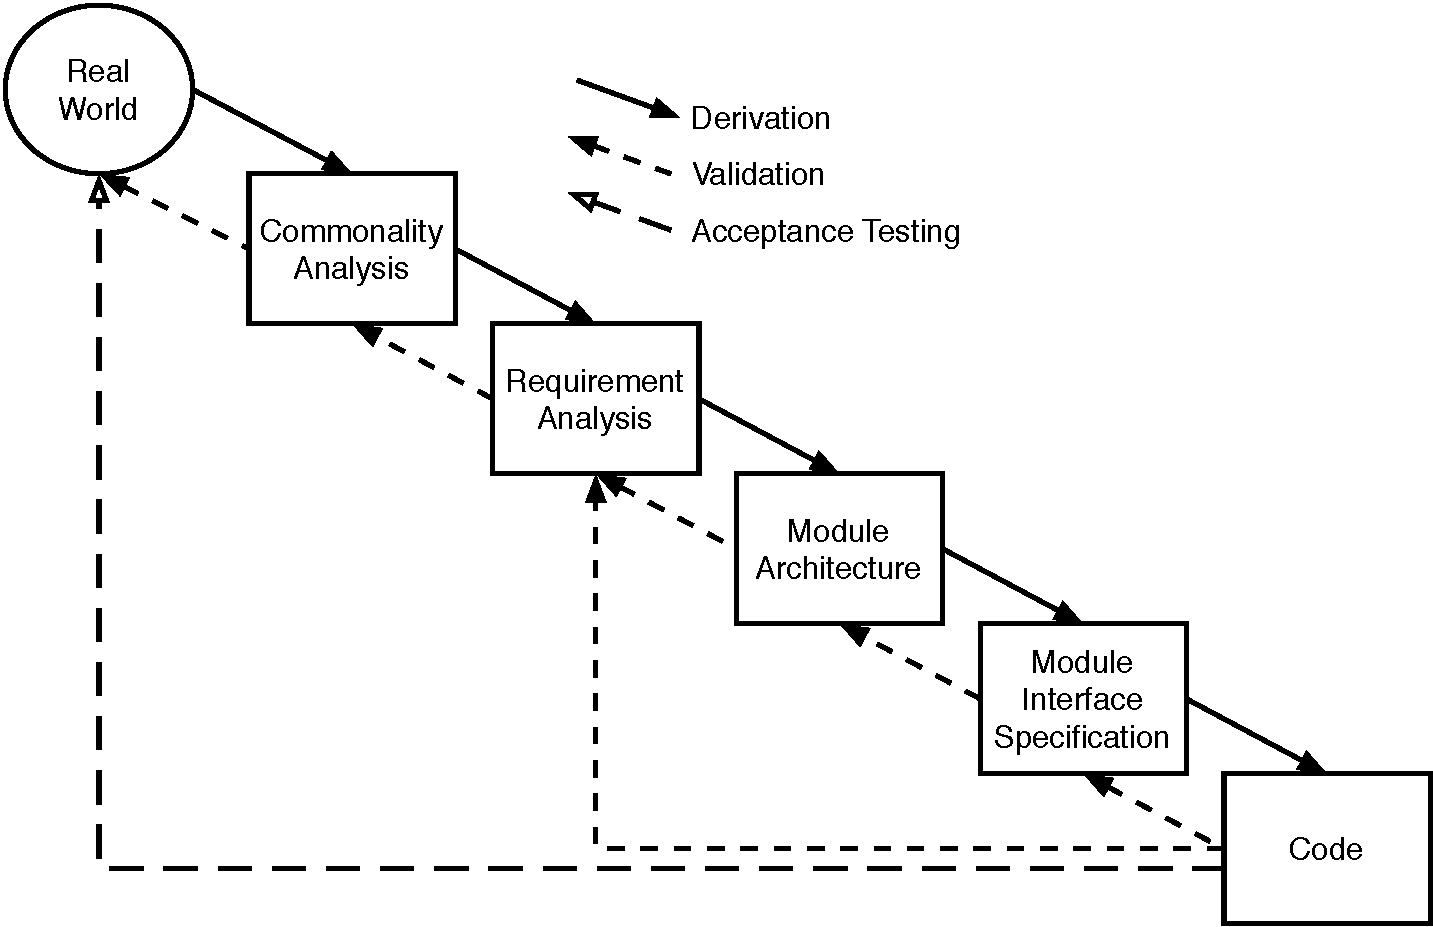
\includegraphics[width=1.0\textwidth]{../Figures/Waterfall.pdf}
\end{center}

\end{frame}

%%%%%%%%%%%%%%%%%%%%%%%%%%%%%%%%%%%%%%%%%%%%%%%%%%%%%%

\begin{frame}

\frametitle{CA to SRS to Design}

\begin{center}
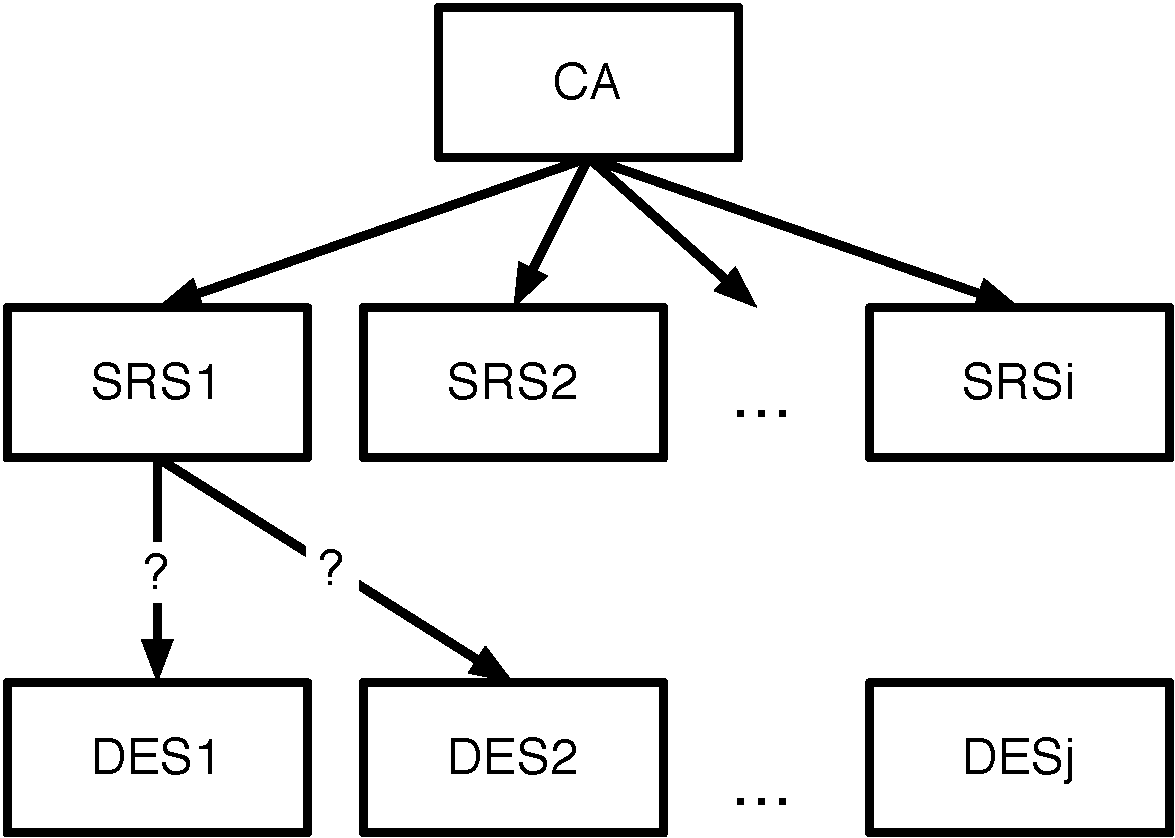
\includegraphics[width=1.0\textwidth]{../Figures/OverviewOfMethodology.pdf}
\end{center}

% mention an overview of what goes in the boxes

\end{frame}

%%%%%%%%%%%%%%%%%%%%%%%%%%%%%%%%%%%%%%%%%%%%%%%%%%%%%%

\begin{frame}

\frametitle{Proposed Methodology}

\begin{enumerate}

\item Identify family of interest
\begin{itemize}
\item Specific physical model?
\item Multipurpose tool?
\end{itemize}
\item Commonality Analysis (CA)
\begin{itemize}
\item Terminology
\item Commonalities
\item Variabilities
\item Parameters of variation
\item Binding time
\end{itemize}
\item Domain Specific Language (DSL)
\item Generation of family members

\end{enumerate}

\end{frame}

%%%%%%%%%%%%%%%%%%%%%%%%%%%%%%%%%%%%%%%%%%%%%%%%%%%%%%

\begin{frame}

\frametitle{CA Template From \cite{Smith2006}}

\scalebox{1.0}{
\begin{minipage}{0.94\columnwidth}
\begin{enumerate}

\item{Reference Material:}
{a) Table of Contents}
{b) Table of Symbols}
{c) Abbreviations and Acronyms}

\item{Introduction:} 
{a) Purpose of the Document}
{b) Organization of the Document}

\item{General System Description:}
{a) \structure{Potential} System Contexts}
{b) \structure{Potential} User Characteristics}
{c) \structure{Potential} System Constraints}

\item Commonalities:
{a) Background Overview}
{b) Terminology Definition}
\structure{c) Goal Statements}
\structure{d) Theoretical Models}

\item \structure{Variabilities:
{a) Input Assumptions}
{b) Calculation}
{c) Output}}

\item \structure{Requirements (added to template)}

%\item \structure{Likely Changes}

\item{Traceability Matrix}

%\item{References}

\end{enumerate}
\end{minipage}
}
% highlight parts to talk about
\end{frame}

%%%%%%%%%%%%%%%%%%%%%%%%%%%%%%%%%%%%%%%%%%%%%%%%%%%%%%

\begin{frame}

\frametitle{Abstract Requirements}

% explain how CAnal addresses this challenge
\begin{itemize}
\item Appropriate level of abstraction by refining from goal to theory to input assumptions
\item A goal is a functional objective the software should achieve: \newline
\structure{\textbf{G1:} Find the roots of an equation}
\item Goals are refined into theoretical models: \newline
% presented as they would be presented in a mathematics textbook 
\structure{\textbf{T1:} Given a function $f(x)$ and an interval $ \{ x | x_{lower} \leq x_{upper} \} $,
return the points where $f(x) = 0$}
\item Introduce simplifying assumptions to allow theoretical model to be solved:\newline
\structure{\textbf{VA1,2:} $f(x)$ is continuous on the interval and/or $f(x)$ has at least one sign change on the
interval}
%traceability matrix?
\end{itemize}
\end{frame}

%%%%%%%%%%%%%%%%%%%%%%%%%%%%%%%%%%%%%%%%%%%%%%%%%%%%%%

\begin{frame}

\frametitle{Abstract Requirements (Continued)}

\begin{itemize}
\item Each variability has an associated parameter of variation and a binding time
\begin{itemize}
\item Specification time
\item Compile time
\item Generation time
\item Run time
\end{itemize}
\end{itemize}
\end{frame}

%%%%%%%%%%%%%%%%%%%%%%%%%%%%%%%%%%%%%%%%%%%%%%%%%%%%%%

\begin{frame}

\frametitle{Capture Existing Knowledge}

\begin{itemize}
\item Systematic consideration from general to specific
\item Communication between experts
\item Standard template allows comparison
\item Convenient framework for summarizing existing literature
\item Eventually a library of requirements documentation
% \item Same goal may have different theoretical models
\item CA refined by a family of SRSs
\end{itemize}
\end{frame}
%%%%%%%%%%%%%%%%%%%%%%%%%%%%%%%%%%%%%%%%%%%%%%%%%%%%%%

\begin{frame}

\frametitle{System Requirements Specification (SRS)}

\begin{itemize}

\item Based on IEEE Standard 830 and Volere requirements specification template
\item Sections from CA are refined in SRS
\item ``Potential'' descriptions are made specific
\item Variabilities are set
\item Binding times are set

\end{itemize}

\end{frame}

%%%%%%%%%%%%%%%%%%%%%%%%%%%%%%%%%%%%%%%%%%%%%%%%%%%%%%

\begin{frame}

\frametitle{SRS Template}

\scalebox{1.0}{
\begin{minipage}{0.94\columnwidth}
\begin{enumerate}

\item{Reference Material}%:
%{a) Table of Contents}
%{b) Table of Symbols}
%{c) Abbreviations and Acronyms}

\item{Introduction}%:
%{a) Purpose of the Document}
%{b) Scope of the Software Product}
%{c) Organization of the Document}

\item{General System Description}%:
%{a) System Context}
%{b) User Characteristics}
%{c) System Constraints}

\item {Specific System Description:}
{a) Background Overview,}
{b) Terminology Definition,}
{c) Goal Statements}
{d) Theoretical Models,}
{e) Assumptions,}
{f) Data Constraints,}
{g) System Behaviour}

\structure{\item Non-functional Requirements:
{a) Accuracy of Input Data,}
{b) Sensitivity of the Model,}
{c) Tolerance of Solution,}
{d) Performance,}
{...}
{i) Portability,}}

\structure {\item {Solution Validation Strategies, (moved to separate document)}}

\item{Other System Issues:}
%{ Open Issues}
%{ Off-the-Shelf Solutions}
%{ New Problems}
%{ Waiting Room}

\item{Traceability Matrix}

%\item List of Possible Changes in the Requirements

%\item{Values of Auxiliary Constants}

%\item{References}

\end{enumerate}
\end{minipage}
}

\end{frame}

%%%%%%%%%%%%%%%%%%%%%%%%%%%%%%%%%%%%%%%%%%%%%%%%%%%%%%

\begin{frame}

\frametitle{NFRs}

\begin{itemize}

\item Rather than absolute quantification of NFRs, use relative comparison between other program family members
\item Specify requirements in big O notation
% makes the requirement validatable
%\item Identify benchmark test problems %system test plan
%\item A posteriori description, rather than a priori specification
\item Relative importance between NFRs using Analytic Hierarchy Process (AHP) \cite{Saaty1980}
\begin{itemize}
\item Addresses challenge of comparing attributes that are measured in different (or hard to quantify) units
\item Series of pair-wise comparisons between attributes
\item 1 for equal importance, 3 for moderately strong importance, ..., 9 for extreme importance
\end{itemize}

\end{itemize}

\end{frame}

%%%%%%%%%%%%%%%%%%%%%%%%%%%%%%%%%%%%%%%%%%%%%%%%%%%%%%

\begin{frame}

\frametitle{Validatable Requirements}

\begin{itemize}

%\item Rather than absolute quantification of NFRs, use relative comparison between other program family members
% makes the requirement validatable
\item Relative comparison between programs is a validatable requirement
\item Focus on a posteriori description, rather than a priori specification
% experiment with the software, as experiment with nature
\item Solution validation strategies
\begin{itemize}
\item Solve using different techniques
\item Identify benchmark test problems %system test plan
\item Test cases built starting from assumed solutions (Method of Manufactured Solutions)
\item Partially validate for a simpler subset where the solution is known
\end{itemize}

\end{itemize}

\end{frame}

%%%%%%%%%%%%%%%%%%%%%%%%%%%%%%%%%%%%%%%%%%%%%%%%%%%%%%

\begin{frame}
\frametitle{Mesh Generating Software}
\begin{figure}
\begin{center}
\rotatebox{0}
{
 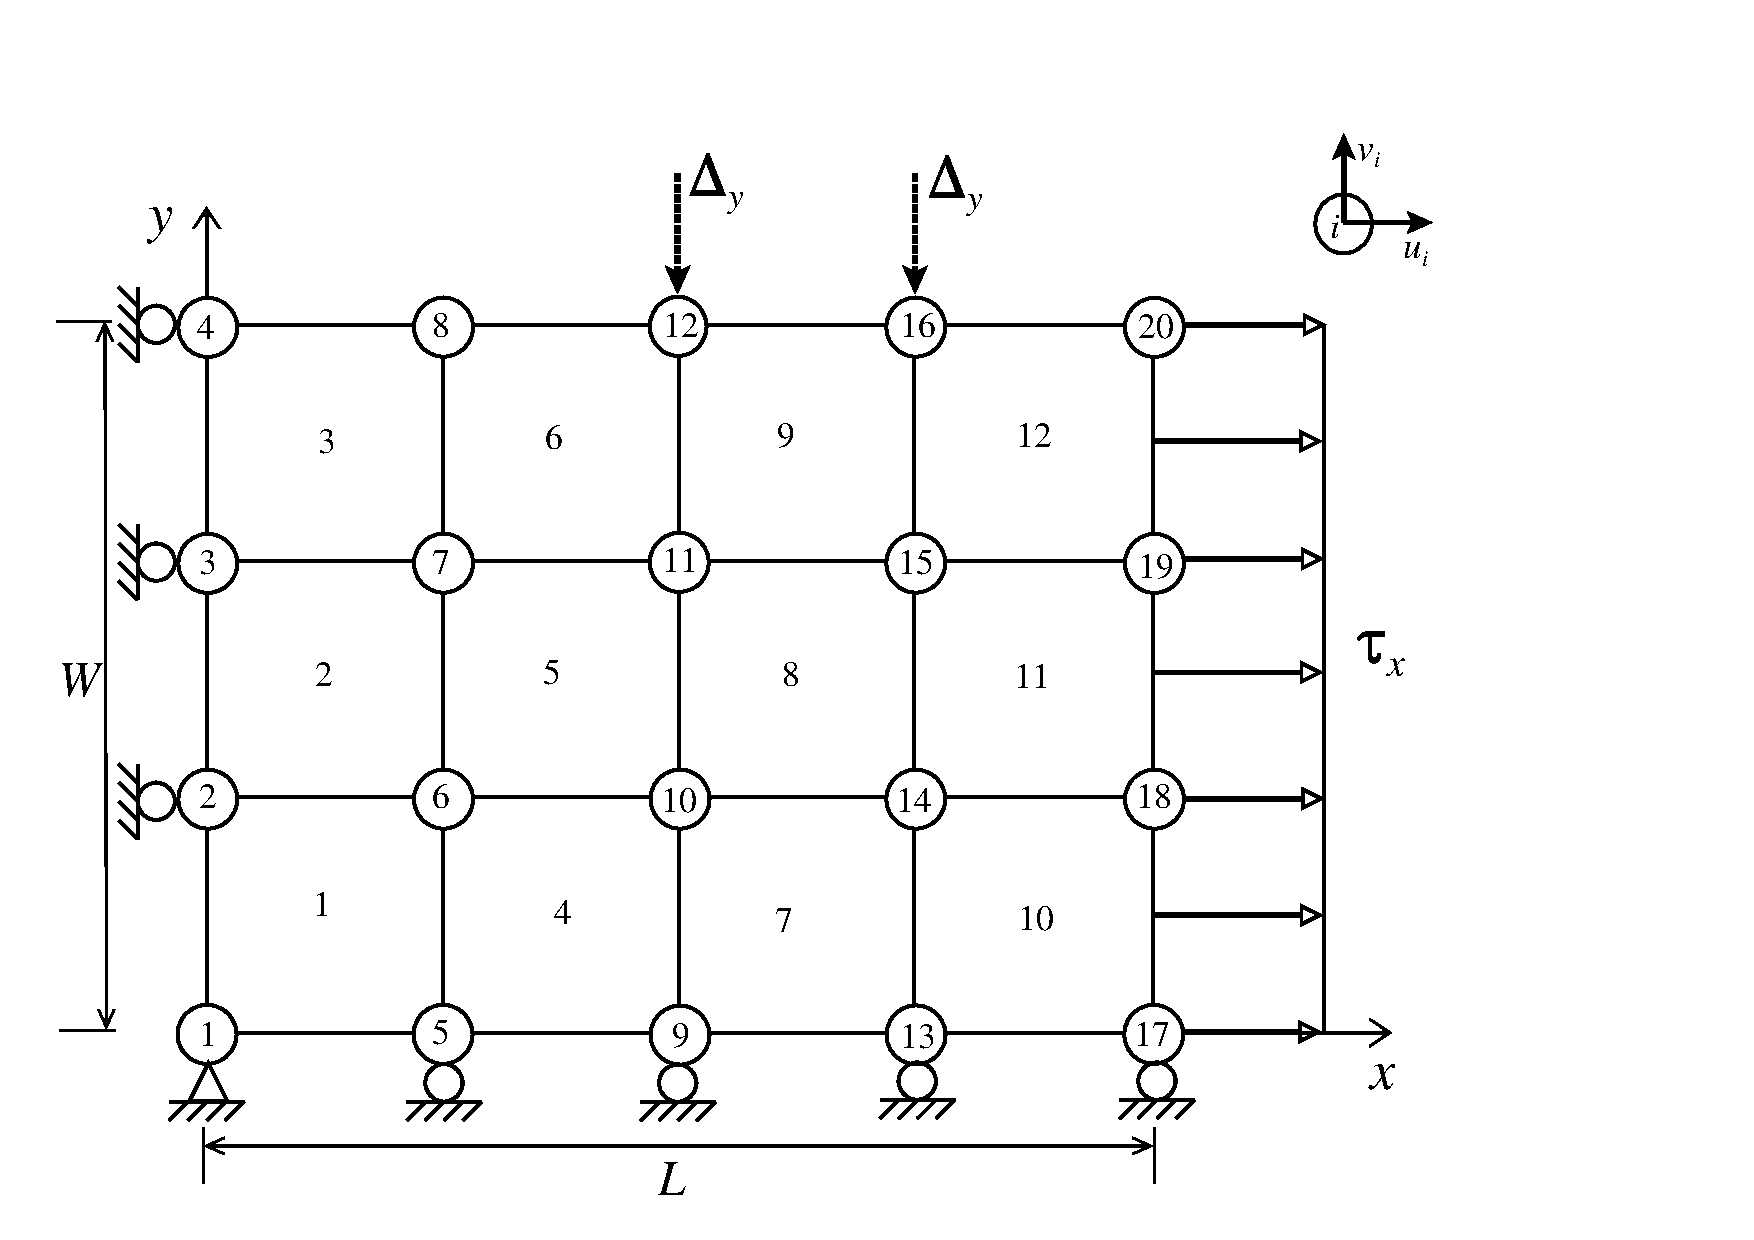
\includegraphics[width=0.9\textwidth]{../Figures/ExampleMesh.pdf}
}
%\caption{Example finite element mesh}
\end{center}
\end{figure}

\end{frame}

%%%%%%%%%%%%%%%%%%%%%%%%%%%%%%%%%%%%%%%%%%%%%%%%%%%%%%

\begin{frame}
\frametitle{Commonality Analysis for a Mesh Generator}

From Chen's work \cite{Chen2003, SmithAndChen2004, SmithAndChen2004b}.
Alternate approach in \cite{BastarricaAndHitschfeld2006, RosselEtAl2014,
  BastarricaAndHitschfeld-Kahler2004,
  Bastarrica2002, BastarricaAndHitschfeld2004}

\begin{itemize}

\item Terminology
\begin{itemize}
\item requirement
\item structured mesh, ...
\end{itemize}

\item Commonalities
\begin{itemize}
\item discretization
\item input from user is required, ...
\end{itemize}

\item Variabilities
\begin{itemize}
\item shape of elements
\item coordinate system used, ...
\end{itemize}

\item Parameters of variation
\begin{itemize}
\item line, triangle, quadrilateral, tetrahedral, hexahedral
\item Cartesian, polar, spherical, ...
\end{itemize}

\end{itemize}

\end{frame}

%%%%%%%%%%%%%%%%%%%%%%%%%%%%%%%%%%%%%%%%%%%%%%%%%%%%%%

\begin{frame}
\frametitle{Definition of a Mesh}
Let $\Omega$ be a closed bounded domain in $\mathbb{R}$ or $\mathbb{R}^2$ or $\mathbb{R}^3$
and let $K$
be a simple shape, such as a line segment in 1D, a triangle or a quadrilateral in 2D, or a tetrahedron or hexahedron
in 3D.  A mesh of $\Omega$, denoted by $\tau$, has the following properties:
\begin{enumerate}
\item $\Omega \approx \cup(K | K \epsilon \tau : K)$, where $\cup$ is first closed and then opened
\item the length of every element $K$, of dimension 1, in $\tau$ is greater than zero
\item the interior of every element $K$, of dimension 2 or greater, in $\tau$ is nonempty
\item the intersection of the interior of two elements is empty
\end{enumerate}
\end{frame}

%%%%%%%%%%%%%%%%%%%%%%%%%%%%%%%%%%%%%%%%%%%%%%%%%%%%%%

\begin{frame}
\frametitle{Example Commonality}

\newcommand{\colACwidth}{0.25\textwidth}
\newcommand{\colBCwidth}{0.7\textwidth}

\begin {tabular}{| p{\colACwidth} | p{\colBCwidth}|}
\hline
{\bf Item Number} & C1\\
\hline
{\bf Description} & A mesh generator discretizes a given computational domain (closed boundary $\Omega$) into a covering
up of a finite number of simpler shapes.\\
\hline
{\bf Related Variability} & V6, V8, V12, V14, V15, V16, V17, V18\\
\hline
{\bf History} & Created - May 7, 2004\\
\hline
\end {tabular}

\end{frame}

%%%%%%%%%%%%%%%%%%%%%%%%%%%%%%%%%%%%%%%%%%%%%%%%%%%%%%
\begin{frame}

\frametitle{Mesh Generator (MG) Goals}

\begin{enumerate}[G1]

\item Input spatial domain $\Omega$ output a mesh $M$ that covers this domain.

\item Transform information on the materials, material properties and the
locations of the different materials

\item Transform information on the boundary condition types, values and locations

\item Transform system information, such as numerical algorithm parameters
%values needed by the subsequent
%processing step (for instance initial time, time step size, degree of implicitness, etc.)

\end{enumerate}

\end{frame}

% TO DO - add a slide for the theoretical model? - no room
% TO DO - mention output file format variability via XSLT? - mention during talk, but no room on slides
%%%%%%%%%%%%%%%%%%%%%%%%%%%%%%%%%%%%%%%%%%%%%%%%%%%%%%

\begin{frame}

\frametitle{Element Variability}

Location of nodes: sequence of LocationT \\
Number of dof at nodes: sequence of $\mathbb{N}$ \\
LocationT = tuple of ($L_1: \mbox{natT}$, $L_2: \mbox{natT}$, $L_3: \mbox{natT}$)\\
natT = \{ $s: \mathbb{R} | 0 \leq s \leq 1 : s$ \}\\

\begin{center}
%\rotatebox{-90}
{
 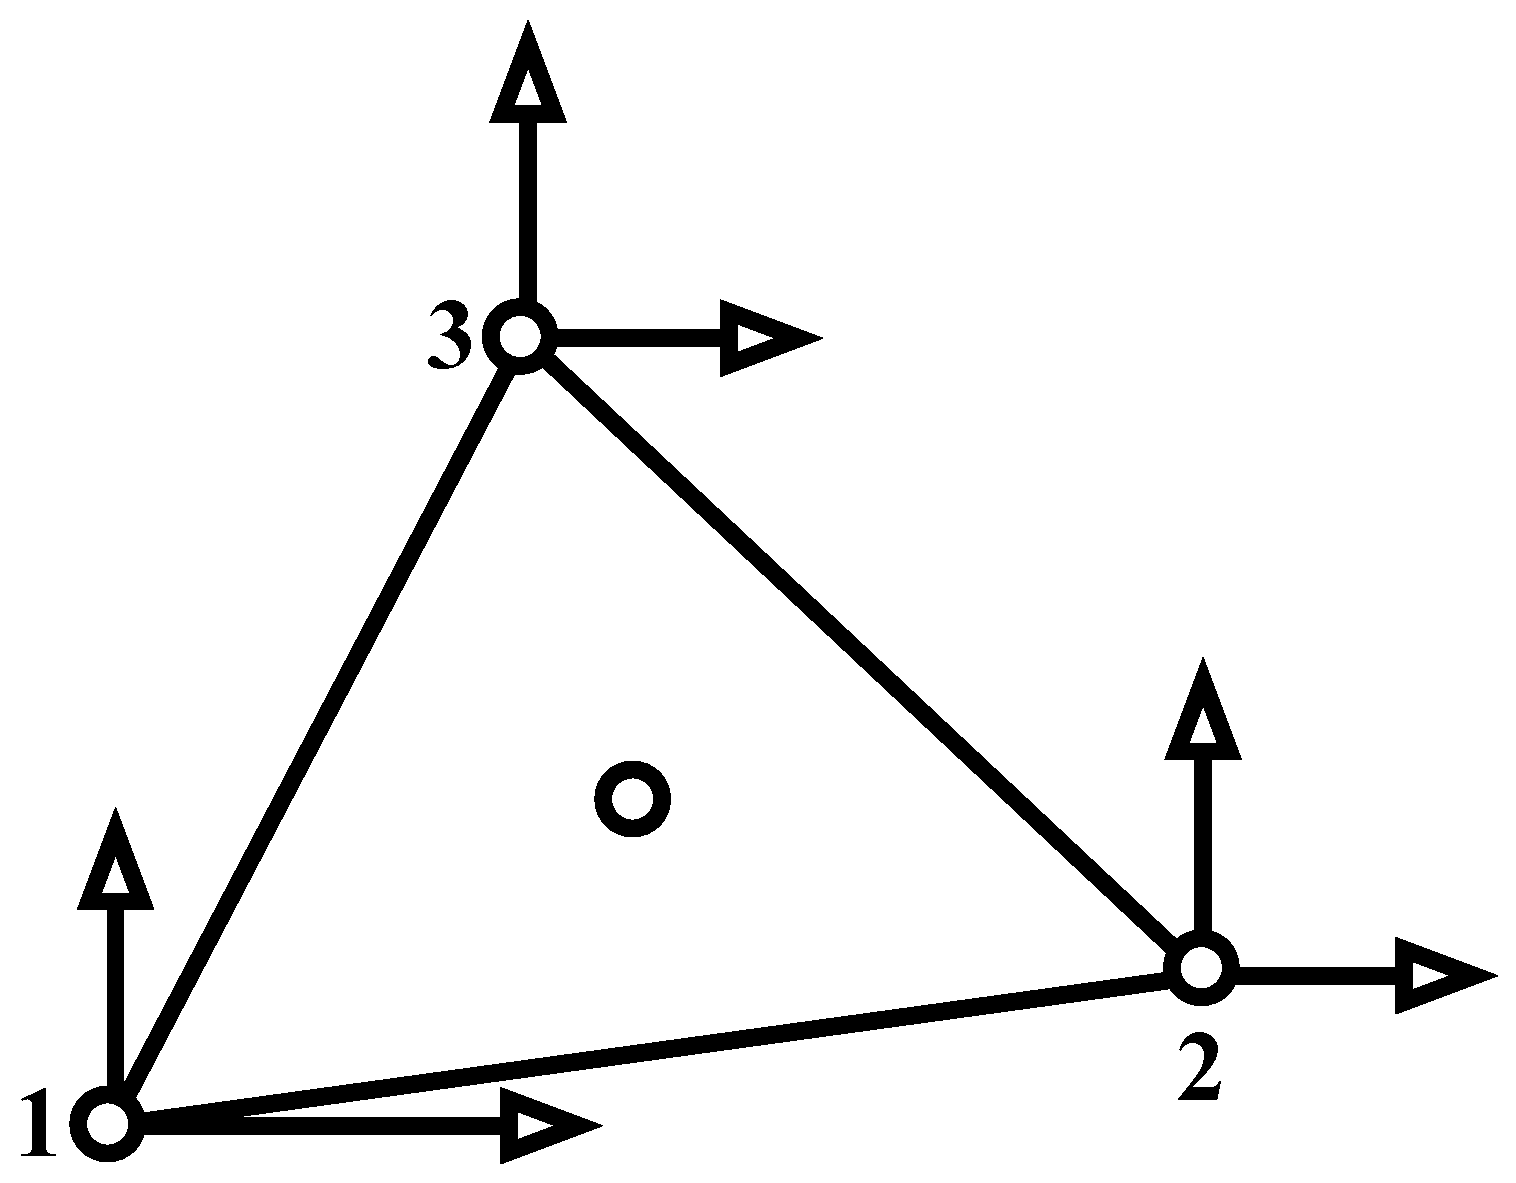
\includegraphics[width=0.5\textwidth]{../Figures/TriangleElement.pdf}
}
\end{center}

\end{frame}

%%%%%%%%%%%%%%%%%%%%%%%%%%%%%%%%%%%%%%%%%%%%%%%%%%%%%%

\begin{frame}

\frametitle{Local Topology Variability}

\begin{center}
{
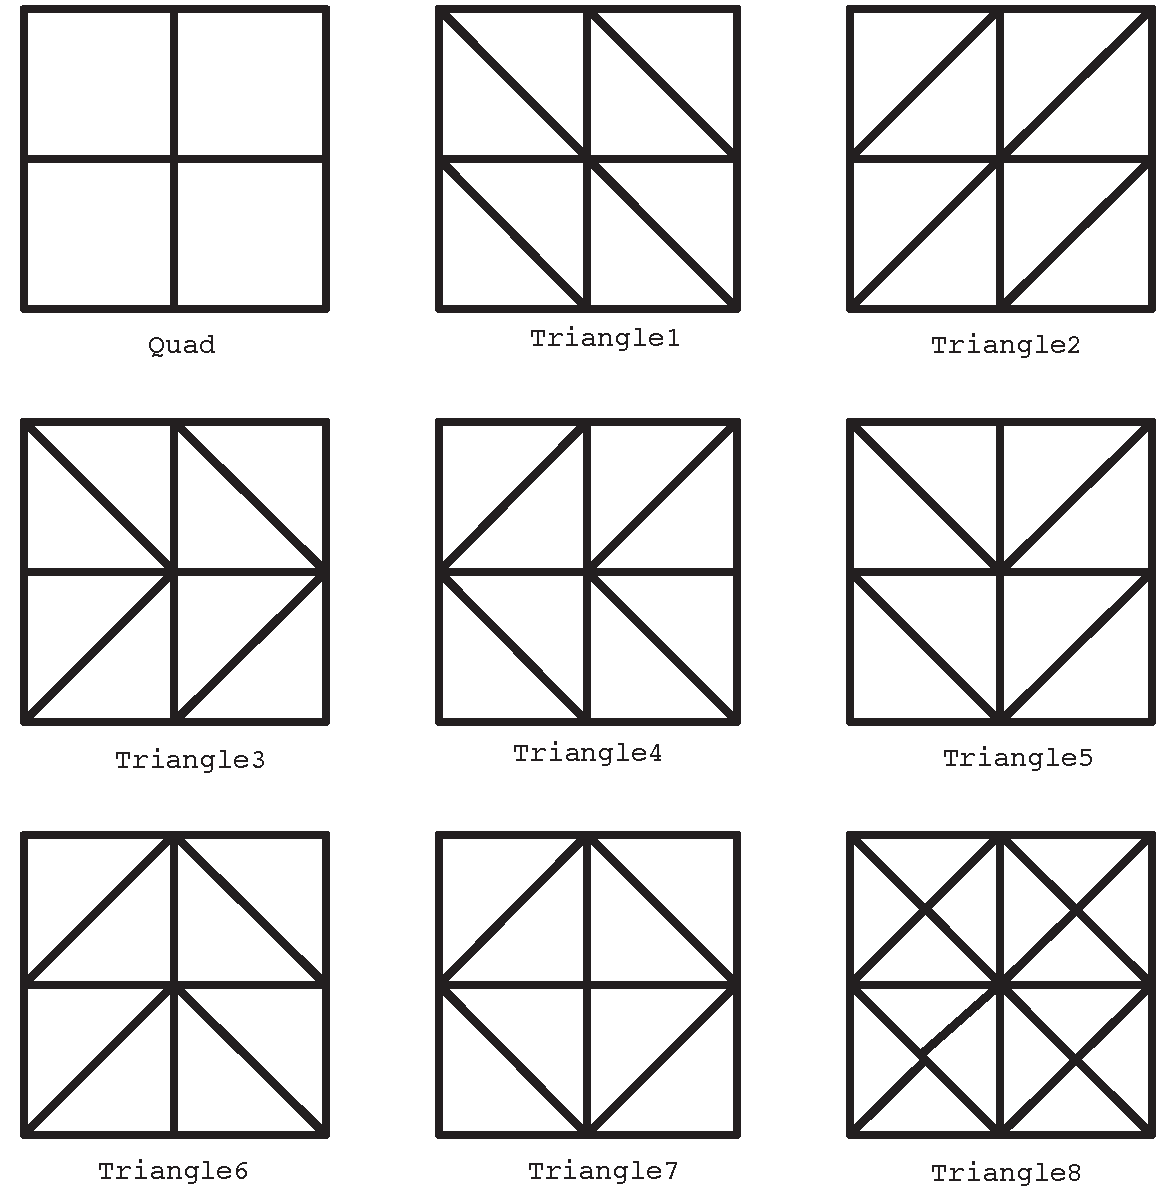
\includegraphics[width=0.65\textwidth]{../Figures/TopologyPatterns.pdf}
}
\end{center}

\end{frame}

%%%%%%%%%%%%%%%%%%%%%%%%%%%%%%%%%%%%%%%%%%%%%%%%%%%%%%

\begin{frame}[fragile]

\frametitle{DSL Using XML}

\lstset{language=XML,linewidth=.9\textwidth,xleftmargin=0.5cm}
\begin{lstlisting}%[frame=single]

<elementSet>
    <geometrySpec>
        <shape>triangle1</shape>
        <nodeGeo count="3">
            <node id="1">
                <location>1,0,0</location>
            </node>
            <node id="2">
                <location>0,1,0</location>
            </node>
            ...
        </nodeGeo>
    </geometrySpec>
</elementSet>
\end{lstlisting}

\end{frame}

%%%%%%%%%%%%%%%%%%%%%%%%%%%%%%%%%%%%%%%%%%%%%%%%%%%%%%

\begin{frame}

\frametitle{Proof of Concept Implementation}

From Cao's work \cite{Cao2006, SmithMcCutchanAndCao2007}
\begin{itemize}
\item XML document that customizes a Java object
\item The Java object customizes the general purpose MG as it is loaded
\item General purpose MG
\begin{itemize}
\item All variabilities bound at run-time
\item Corresponds to an empty XML specification
\end{itemize}
\end{itemize}

\begin{center}
{
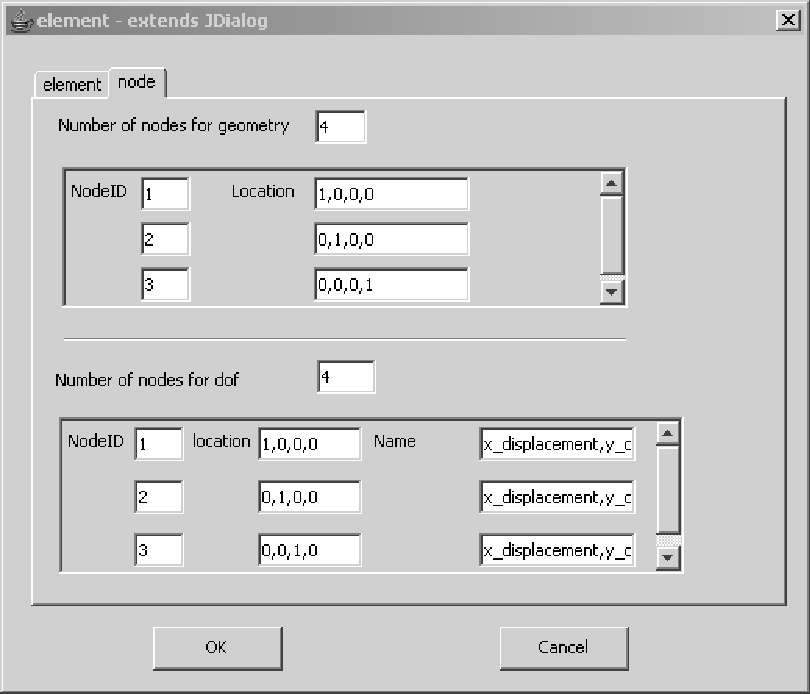
\includegraphics[width=0.4\textwidth]{../Figures/elementdialog2.png}
}
\end{center}

\end{frame}

%%%%%%%%%%%%%%%%%%%%%%%%%%%%%%%%%%%%%%%%%%%%%%%%%%%%%%

\begin{frame}
\frametitle{Linear Systems of Equations}

$$A x = b$$

Commonality analysis presented in \cite{Smith2006}

\end{frame}

%%%%%%%%%%%%%%%%%%%%%%%%%%%%%%%%%%%%%%%%%%%%%%%%%%%%%%

%\begin{frame}

%\frametitle{Terminology}

%\begin{tabular}{ l p{5.5cm}}
%$n: \mathbb{N}$ & number of linear equations and the number of unknowns\\
%$A: \mathbb{R}^{n \times n}$ & $n \times n$ real matrix\\
%$x: \mathbb{R}^{n \times 1}$ & $n \times 1$ real column vector\\
%$b: \mathbb{R}^{n \times 1}$ & $n \times 1$ real column vector\\
%$I: \mathbb{R}^{n \times n}$ & an $n \times n$ matrix where all entries are $0$, except for the diagonal entries, which
%are $1$\\
%$A^{-1}: \mathbb{R}^{n \times n}$ & the inverse matrix, with the property that $A^{-1} A = I$\\
%$|| v || $ & the norm (estimate of magnitude) of vector $v$\\
%residual & $|| b - A x ||$\\
%singular & matrix $A$ is singular if $A^{-1}$ does not exist\\
%\end{tabular}

%\end{frame}

%%%%%%%%%%%%%%%%%%%%%%%%%%%%%%%%%%%%%%%%%%%%%%%%%%%%%%

\begin{frame}

\frametitle{Goal and Theoretical Model}

\textbf{G1}: Given a system of $n$
linear equations represented by matrix $A$ and column vector $b$, return $x$ such that $A x = b$, if possible

\textbf{T1}: Given square matrix $A$ and column vector $b$, the possible
solutions for $x$ are as follows:

\begin{enumerate}
\item A unique solution $x = A^{-1} b$, if $A$ is nonsingular
\item An infinite number of solutions if $A$ is singular and $b \in span(A)$
\item No solution if $A$ is singular and $b \notin span(A)$
\end{enumerate}

\end{frame}

%%%%%%%%%%%%%%%%%%%%%%%%%%%%%%%%%%%%%%%%%%%%%%%%%%%%%%

\begin{frame}

\frametitle{Variabilities for Input Assumptions}

\begin{tabular}{| p{\colA} | p{\colB} | }
\hline
\textbf{Variability} & \textbf{Parameter of Variation} \\
\hline
Allowed structure  $A$ & Set of \{ full, sparse, banded, tridiagonal, block triangular, ...,
%block structured, diagonal, upper triangular, lower triangular, 
Hessenberg \} \\
\hline
Allowed definiteness $A$ & Set of \{ not definite, positive definite, ...,
%positive semi-definite, negative definite, 
negative semi-definite \} \\
\hline
Allowed class of $A$ & Set of \{ diagonally dominant, Toeplitz, Vandermonde \} \\
\hline
Symmetry\newline assumed? & boolean \\
\hline
Possible values for $n$ & set of $\mathbb{N}$ \\
\hline
Possible entries in $A$ & set of $\mathbb{R}$ \\
\hline
... & ... \\
%Possible entries in $b$ & set of $\mathbb{R}$ \\
%\hline
%Source\newline of input & Set of \{ from a file, through the user interface, passed in memory \} \\
%\hline
%Encoding of input & Set of \{binary, text \} \\
%\hline
%Format\newline of input $A$ & Set of \{arbitrary, by row, by column, by diagonal \} \\
%\hline
%Format\newline of input $b$ & Set of \{arbitrary, ordered \} \\\hline
\end{tabular}

\end{frame}

%%%%%%%%%%%%%%%%%%%%%%%%%%%%%%%%%%%%%%%%%%%%%%%%%%%%%%

\begin{frame}

\frametitle{Variabilities for Calculation}

\begin{tabular}{| p{\colA} | p{\colB} | }
\hline
\textbf{Variability} & \textbf{Parameter of Variation} \\
\hline
Check input? & boolean (false if the input is assumed to satisfy the input assumptions)\\ 
\hline
Exceptions generated? & boolean (false if the goal is non-stop arithmetic)\\ 
\hline
Norm used for residual & Set of \{1-norm, 2-norm, $\infty$-norm \} \\
\hline
\end{tabular}

% mention turning off input checking helps with problem of theoretical model refined by assumpts

\end{frame}

%%%%%%%%%%%%%%%%%%%%%%%%%%%%%%%%%%%%%%%%%%%%%%%%%%%%%%

\begin{frame}

\frametitle{Variabilities for Output}

\begin{tabular}{| p{\colA} | p{\colB} | }
\hline
\textbf{Variability} & \textbf{Parameter of Variation} \\
\hline
Destination for output $x$ & Set of \{ to file, to screen, to memory \} \\
\hline
Encoding of output $x$ & Set of \{binary, text \} \\
\hline
Format of output $x$ & Set of \{arbitrary, ordered \} \\
\hline
Output residual & boolean (true if the program returns the residual) \\
\hline
Possible entries in $x$ & set of $\mathbb{R} \cup \{- \infty, \infty, undef \}$ \\
\hline
\end{tabular}

\end{frame}

%%%%%%%%%%%%%%%%%%%%%%%%%%%%%%%%%%%%%%%%%%%%%%%%%%%%%%

\begin{frame}

\frametitle{Analytic Hierarchy Process}

\begin{itemize}
\item Example 1
\begin{itemize}
\item Embedded real-time system for digital signal processing
\item $n = 10$
\item $A$ is assumed to be Toeplitz
\end{itemize}
\end{itemize}

\begin{tabular}{| l | l | l | l | l |}
\hline
~ & \textbf{Speed} & \textbf{Accuracy} & \textbf{Portability} & \textbf{Priority}\\
\hline
\textbf{Speed} & 1 & 3 & 5 & 0.64\\
\textbf{Accuracy} & 1/3 & 1 & 3 & 0.26\\
\textbf{Portability} & 1/5 & 1/3 & 1 & 0.11\\
\hline
\end{tabular}

\end{frame}

%%%%%%%%%%%%%%%%%%%%%%%%%%%%%%%%%%%%%%%%%%%%%%%%%%%%%%

%\begin{frame}

%\frametitle{AHP Continued}

%\begin{itemize}
%\item Example 2
%\begin{itemize}
%\item Structural mechanics software for education
%\item $10 \leq n \leq 1000$
%\item $A$ is assumed to be positive definite
%\item Would have different relative priorities
%\end{itemize}
%\end{itemize}

%\end{frame}

%%%%%%%%%%%%%%%%%%%%%%%%%%%%%%%%%%%%%%%%%%%%%%%%%%%%%%

\begin{frame}

\frametitle{Solution Validation Strategies (for VnV Plan)}

\begin{itemize}
\item Create test cases with known solutions
\begin{itemize}
\item Assume $A$ and $x$, calculate $b$
\item Given $A$ and $b$ calculate $x^*$ and compare to the assumed $x$
\end{itemize}
\item Comparison with Matlab
\item Comparison with NAG library
\item Where possible compare solution to interval arithmetic solution
\item Experiments to describe how accuracy changes with increasing condition number
\end{itemize}

\end{frame}

%%%%%%%%%%%%%%%%%%%%%%%%%%%%%%%%%%%%%%%%%%%%%%%%%%%%%%

\begin{frame}

\frametitle{Connection to Design}

\begin{itemize}

\item Abstract requirements to concrete design decisions
%\item Software packages likely already exist within the program family
\item Reuse existing packages within the program family
\item Summarize existing software by the parameters of variation and binding time
%\item Run time binding can often be changed to specification time binding
\item If functional requirements match, then use NFRs
\begin{itemize}
\item AHP to compare each design against each of the NFRs %as done in SRS 
%cols and rows are des alternatives, compared against a given NFR
%repeat for each NFR
\item Contribution of each NFR for each design alternative is found by multiplying the contribution of
each alternative to the given NFR with the corresponding priority of that NFR
\item Sum the contributions
\item The highest overall score is the ``winning'' alternative
\end{itemize}

\end{itemize}

\end{frame}

%%%%%%%%%%%%%%%%%%%%%%%%%%%%%%%%%%%%%%%%%%%%%%%%%%%%%%

\begin{frame}

\frametitle{A Family of Material Models}

From McCutchan's work \cite{CaretteEtAl2008, SmithMcCutchanAndCao2007,
  SmithEtAl2008, CaretteEtAl2007_TR, SmithMcCutchanAndCarette2017, McCutchan2007}

\begin{center}
{
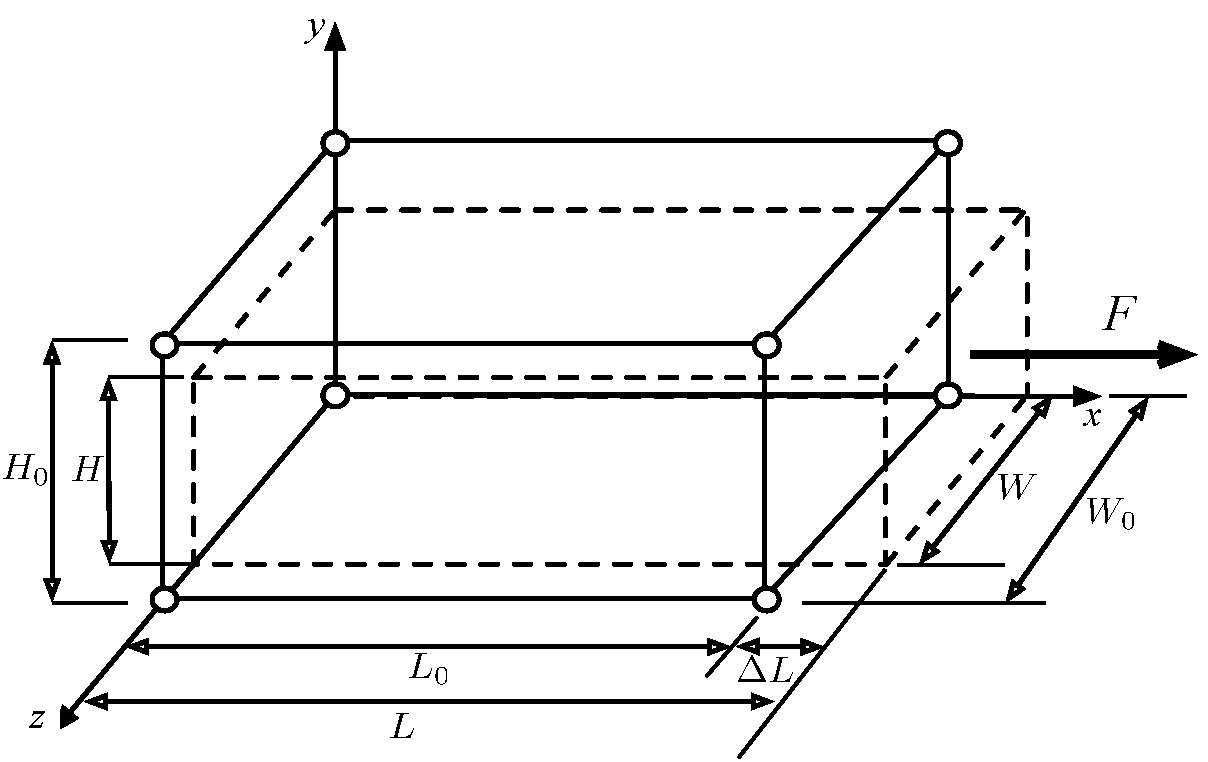
\includegraphics[width=0.5\textwidth]{../Figures/TestSpecimenUniaxial.pdf}
}
\end{center}

\begin{center}
\begin{tabular}{cc}
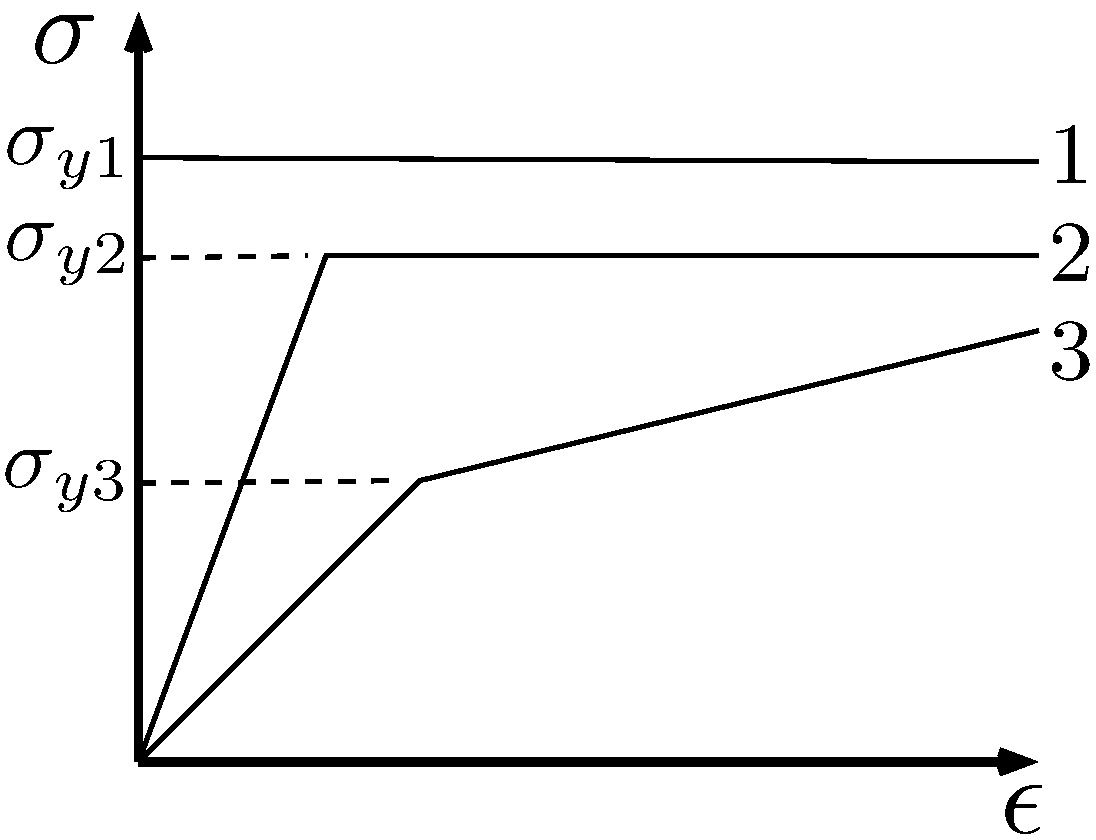
\includegraphics[width=0.45\textwidth]{../Figures/Plastic.pdf} &
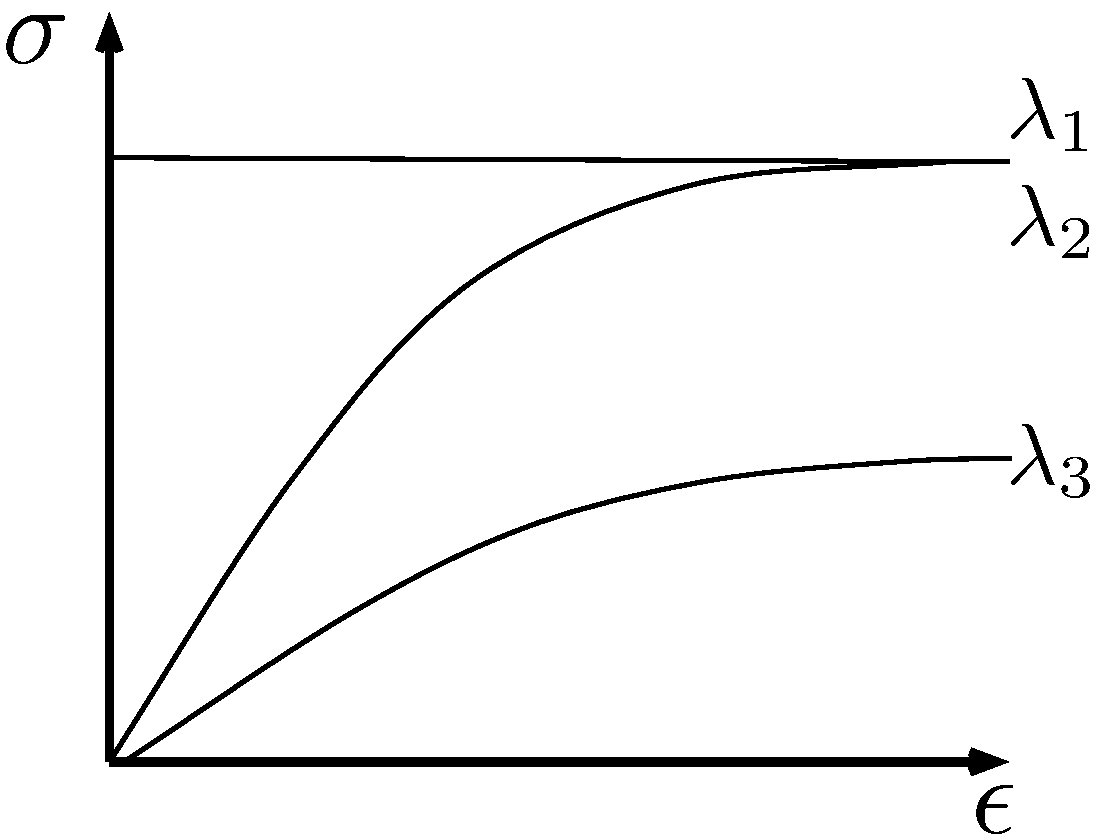
\includegraphics[width=0.45\textwidth]{../Figures/Viscoplastic.pdf}\\
\end{tabular}
\end{center}

\end{frame}

%%%%%%%%%%%%%%%%%%%%%%%%%%%%%%%%%%%%%%%%%%%%%%%%%%%%%%

\begin{frame}

\frametitle{Terminology Definitions}

\begin{minipage}{\textwidth}
\begin{tabular}{| p{\colAwidth} | p{\colBwidth}|}
\hline
\rowcolor[gray]{0.9}
Label: & D\_YieldFunction\\ \hline
Symbol: & $F = F(\bm{\sigma}, \kappa)$\\ \hline
Type: & $(\mbox{tensor2DT} \times \mathbb{R}) \rightarrow \mathbb{R}$\\ \hline
%Units: & --\\ \hline
Related: & {D\_Stress}, {D\_HardeningParameter}\\ \hline %originally related items, shorted for space
Sources: & ...\\
\hline Descrip: & The yield function defines a surface $F = 0$ in the six dimensional stress space ...\\
%\hline History: & Created -- June 15, 2007\\
\hline
\end{tabular}
\end{minipage}

\begin{center}
{
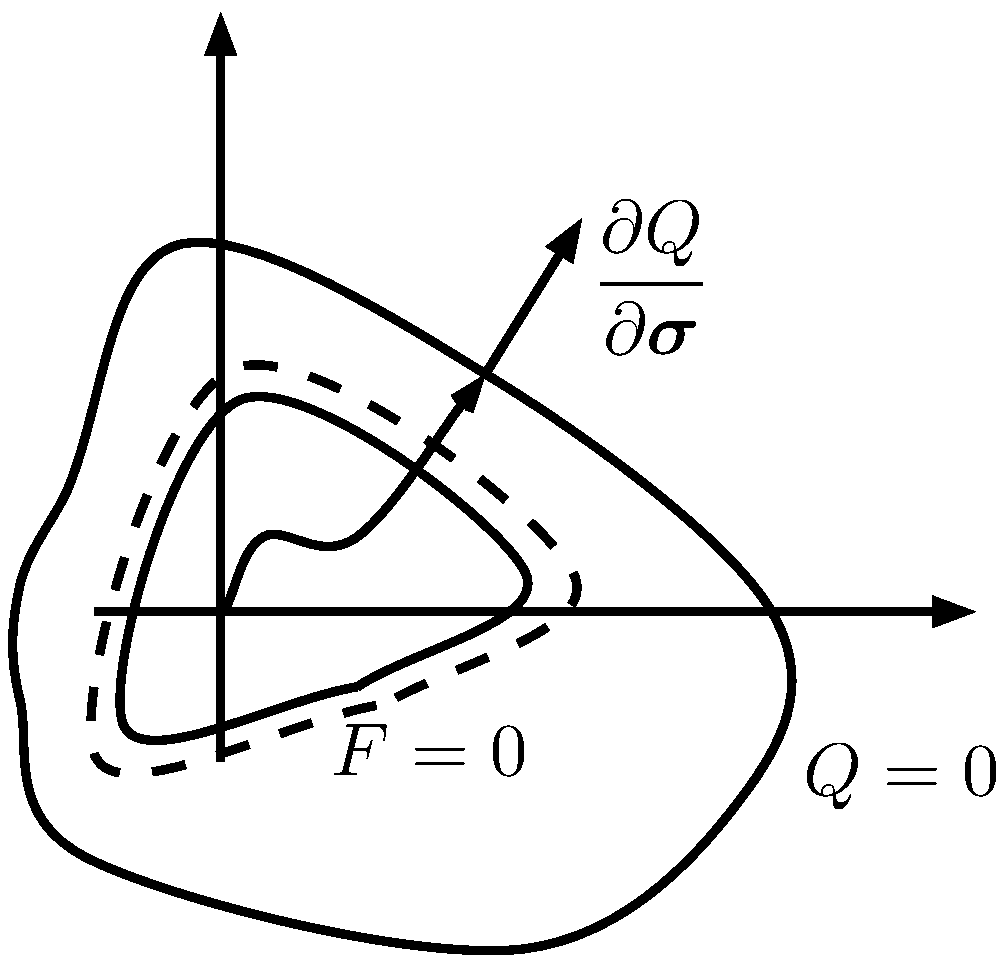
\includegraphics[width=0.35\textwidth]{../Figures/YieldHardeningAndPlastPotential.pdf}
}
\end{center}

\end{frame}

%%%%%%%%%%%%%%%%%%%%%%%%%%%%%%%%%%%%%%%%%%%%%%%%%%%%%%

\begin{frame}

\frametitle{Goal Statement}

\noindent
\begin{minipage}{\textwidth}
\begin{tabular}{| p{\colAwidth} | p{\colBwidth}|}
\hline
\rowcolor[gray]{0.9}
Label: & G\_StressDetermination\\ \hline
Descrip: & Given the initial stress and the deformation history of a material particle, determine the stress
within the material particle.\\
\hline
Refine: & {T\_ConstitEquation}\\ \hline
%History: & Created -- June 8, 2007\\ \hline
\end{tabular}
\end{minipage}

\begin{center}
{
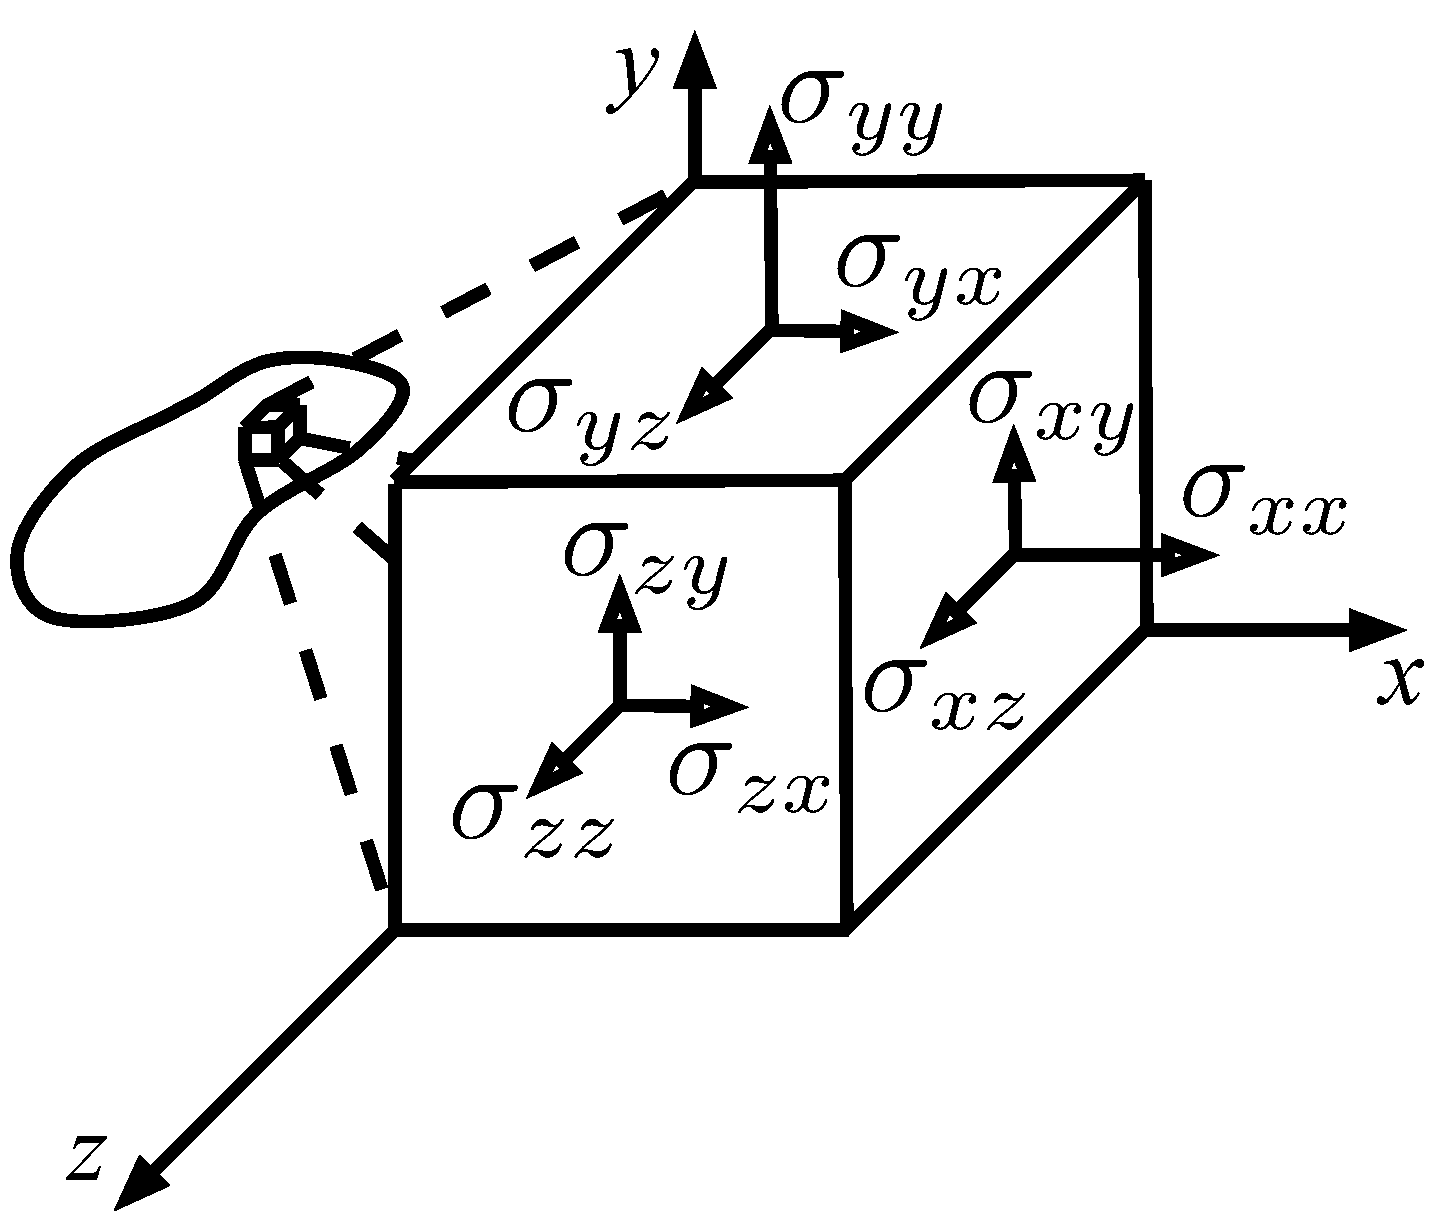
\includegraphics[width=0.5\textwidth]{../Figures/StressTensor.pdf}
}
\end{center}

\end{frame}

%%%%%%%%%%%%%%%%%%%%%%%%%%%%%%%%%%%%%%%%%%%%%%%%%%%%%%

\begin{frame}

\frametitle{Assumptions}

\begin{minipage}{\textwidth}
\begin{tabular}{| p{\colAwidth} | p{\colBwidth}|}
\hline
\rowcolor[gray]{0.9}
Label: & A\_AdditivityPostulate\\ \hline
Related: & {D\_StrainRate}\\ \hline
Equation: & $\dot{\bm{\epsilon}} = \dot{\bm{\epsilon}}^e + \dot{\bm{\epsilon}}^{\mathit{vp}}$\newline
with the following types and units\newline
$\dot{\bm{\epsilon}}: \mbox{tensor2DT}$ (1/t) (1/s)\newline
$\dot{\bm{\epsilon}}^e: \mbox{tensor2DT}$ (1/t) (1/s)\newline
$\dot{\bm{\epsilon}}^{\mathit{vp}}: \mbox{tensor2DT}$ (1/t) (1/s)\\ \hline
Descrip: & The total strain rate ($\dot{\bm{\epsilon}}$) is assumed to decompose into elastic
($\dot{\bm{\epsilon}}^e$) and viscoplastic ($\dot{\bm{\epsilon}}^{\mathit{vp}}$)
strain rates.\\ \hline 
Rationale & This is a standard assumption for elastoplastic and elastoviscoplastic materials.  The 
appropriateness of this assumption is born out by the success of theories built upon it.\\ \hline
Source: & [6, page 339]; [7, page 181]\\ \hline %references hard-coded
%History: & Created -- June 11, 2007\\ \hline
\end{tabular}
\end{minipage}

\end{frame}

%%%%%%%%%%%%%%%%%%%%%%%%%%%%%%%%%%%%%%%%%%%%%%%%%%%%%%

\begin{frame}

\frametitle{Theoretical Model}

\begin{minipage}{\textwidth}
\begin{tabular}{| p{\colAwidth} | p{\colBwidth}|}
\hline
\rowcolor[gray]{0.9}
Label: & T\_ConstitEquation\\
\hline
Related: & {A\_CauchyStress}, {A\_DeformationHistory}, {A\_PerzynaConstit}, {A\_AdditivityPostulate},
{A\_ElasticConstit}, {A\_DescriptionOfMotion}, {V\_MaterialProperties}\\
\hline
Input: & $\bm{\sigma}_0: \mbox{tensor2DT}$ (StressU) (Pa)\newline
$t_{\mathit{begin}}: \mathbb{R}$ (t) (s) \newline
$t_{\mathit{end}}: \mathbb{R} $ (t) (s) \newline
$\dot{\bm{\epsilon}}(t) : \{ t: \mathbb{R} | t_{\mathit{begin}} \leq t \leq t_{\mathit{end}} : t \} \rightarrow
\mbox{   } \mbox{   } \mbox{  tensor2DT}$ (1/t) (1/s)\newline
$\mathit{mat\_prop\_val}: \mbox{string} \rightarrow \mathbb{R}$\newline
$E: \mathbb{R}^{+}$ (StressU) (Pa)\newline
$\nu: \mbox{poissonT}$ (dimensionless)
\\
\hline
\end{tabular}
\end{minipage}

\end{frame}

%%%%%%%%%%%%%%%%%%%%%%%%%%%%%%%%%%%%%%%%%%%%%%%%%%%%%%

\begin{frame}

\frametitle{Theoretical Model Continued}

\begin{minipage}{\textwidth}
\begin{tabular}{| p{\colAwidth} | p{\colBwidth}|}
\hline
\rowcolor[gray]{0.9}
Label: & T\_ConstitEquation\\
\hline
Output: & $\bm{\sigma}(t): \{ t: \mathbb{R} | t_{\mathit{begin}} \leq t \leq t_{\mathit{end}} : t \} \rightarrow
\mbox{tensor2DT}$ such that 
$$\dot{\bm{\sigma}} = \mathbf{D} \left ( \dot{\bm{\epsilon}} - \gamma < \phi (F(\bm{\sigma},\kappa) ) >
\frac {
\partial Q (\bm{\sigma})}{
\partial \bm{\sigma}} \right )
$$ 
and $\bm{\sigma}(t_{\mathit{begin}}) = \bm{\sigma}_0$,
the components of $\bm{\sigma}$ have the units of StressU (Pa)\\
\hline
Derive: & The governing differential equation is found by first solving for $\dot{\bm{\epsilon}}^e$
in {A\_AdditivityPostulate} and then ...\\
\hline
Descrip: & The theoretical model is only completely defined once the associated
variabilities~({V\_MaterialProperties}) that define the
material have been set.  ...\\
\hline History: & Created -- June 14, 2007\\
\hline
\end{tabular}
\end{minipage}

\end{frame}

%%%%%%%%%%%%%%%%%%%%%%%%%%%%%%%%%%%%%%%%%%%%%%%%%%%%%%

\begin{frame}

\frametitle{Variabilities}

\begin{itemize}
\item $F = F(\bm{\sigma}, \kappa): \mathbb{R}^6 \times \mathbb{R} \rightarrow \mathbb{R}$
\item $Q = Q(\bm{\sigma}): \mathbb{R}^6 \rightarrow \mathbb{R}$
\item $\kappa = \kappa(\bm{\epsilon}^{\mathit{vp}}): \mathbb{R}^6 \rightarrow \mathbb{R}$
\item $\phi = \phi(F): \mathbb{R} \rightarrow \mathbb{R}$
\item $\gamma: \mathbb{R}$
\item $\mathit{mat\_prop\_names}: \mbox{set of string}$
\end{itemize}

\end{frame}

%%%%%%%%%%%%%%%%%%%%%%%%%%%%%%%%%%%%%%%%%%%%%%%%%%%%%%

\begin{frame}

\frametitle{Dependency Graph} %between commonalities

\begin{center}
{
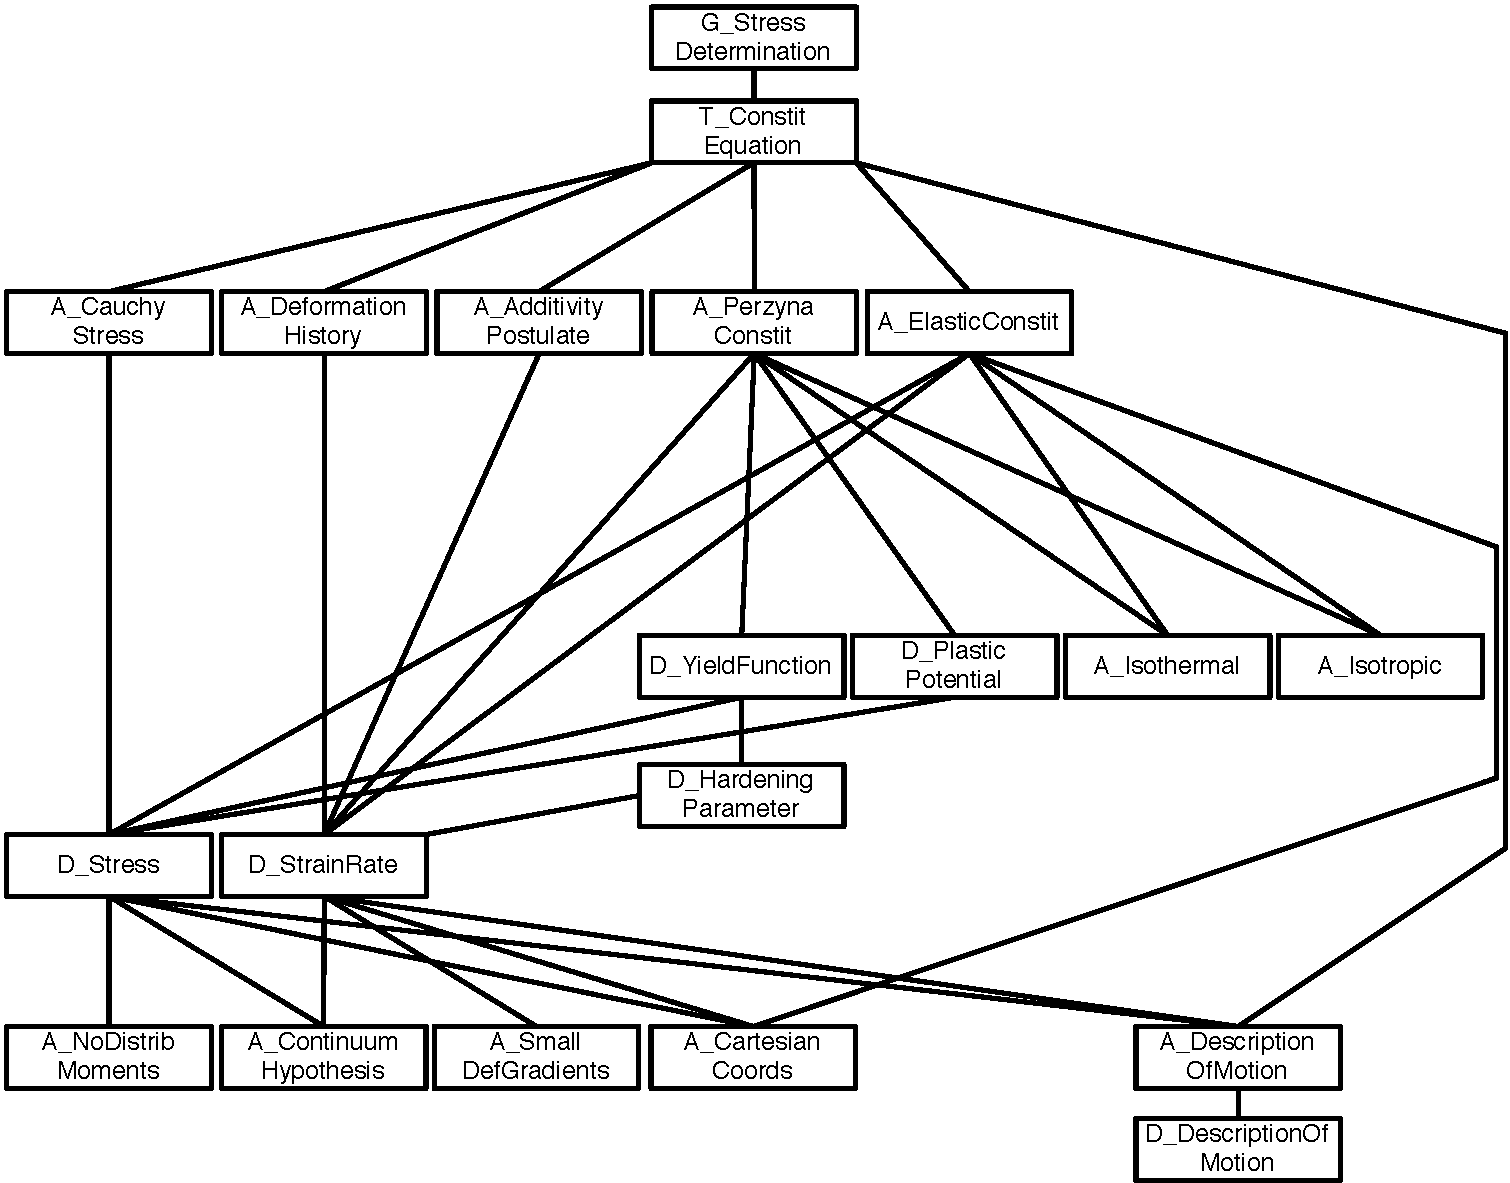
\includegraphics[width=1\textwidth]{../Figures/DependenceGraph.pdf}
}
\end{center}

\end{frame}

%%%%%%%%%%%%%%%%%%%%%%%%%%%%%%%%%%%%%%%%%%%%%%%%%%%%%%

\begin{frame}

\frametitle{Dependency Graph Between Commonalities and Variabilities}

\begin{center}
{
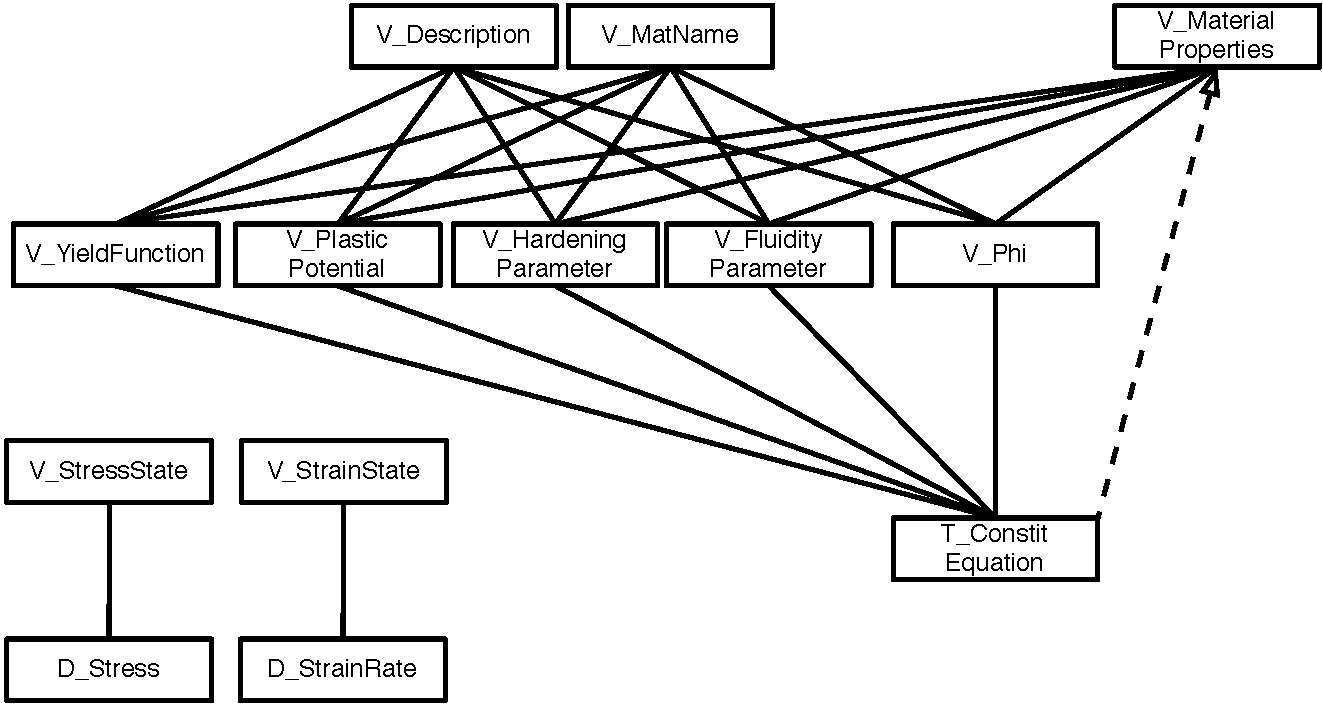
\includegraphics[width=1\textwidth]{../Figures/DependenceOfVariabilities.pdf}
}
\end{center}

\end{frame}

%%%%%%%%%%%%%%%%%%%%%%%%%%%%%%%%%%%%%%%%%%%%%%%%%%%%%%

\begin{frame}

\frametitle{Example}

\begin{minipage}{\textwidth}
\begin{tabular}{| p{0.24\textwidth} | p{0.65\textwidth}|}
\hline
\rowcolor[gray]{0.9}
Label: & E\_StrainHardening\\ \hline
{V\_MatName} & $\mathit{name = }$``Strain-Hardening Viscoelastic''\\
\hline
{V\_YieldFunct} & $F =  q \kappa^{\frac{n-1}{m}}$ (StressU) (Pa)\\ \hline
{V\_PlasticPot} & $Q = q$ (StressU) (Pa)\\ \hline 
{V\_HardParam} & $\kappa = \epsilon_q^{\mathit{vp}}$ (L/L) (m/m)\\
\hline
{V\_Phi} & $\phi = F^{\frac{m}{n}}$ ($\mbox{StressU}^{\frac{m}{n}}$) ($\mbox{Pa}^{\frac{m}{n}}$)\\
\hline
{V\_FluParam} & $\gamma = n A^{\frac{1}{n}}$ ($\mbox{StressU}^{-m} \mbox{t}^{-1}$) ($\mbox{Pa}^{-m} \mbox{s}^{-1}$)\\ \hline
{V\_MatProps} & $\mathit{mat\_prop\_names} = $ \{``$A$'', ``$m$'', ``$n$'' \}, where the type of the
material properties are ...\\
%There is likely an upper limit on the values for $m$ and $n$, but at this time the value of these limits is unclear. 
%With respect to units, $m$ and $n$ do not have units and $A$ has units of $\mbox{StressU}^{-m} \mbox{t}^{-1}$ ($\mbox{Pa}^{-m}%%
%\mbox{s}^{-1}$)
\hline
{V\_Description} & $\mathit{descript =}$ ``This constitutive equation combines a power-law viscoelastic
material with a strain hardening (softening) material.  ...''
\\ \hline
%Source & \cite{Smith2001}
%\\ \hline
%History & Created -- Sept 21, 2007\\ \hline
\end{tabular}
\end{minipage}

\end{frame}

%%%%%%%%%%%%%%%%%%%%%%%%%%%%%%%%%%%%%%%%%%%%%%%%%%%%%%

\begin{frame}

\frametitle{Code Generation}

\begin{itemize}
\item Specify variabilities
\item Symbolically calculate terms needed by numerical algorithm, including $\frac{ \partial Q}{ \partial
\bm{\sigma}}$, $\frac{\partial F}{\partial \bm{\sigma}}$, etc.
\item Symbolic processing avoids tedious and error-prone hand calculations
\begin{itemize}
\item Reduces workload
\item Allows non-experts to deal with new problems
\item Increases reliability
\end{itemize}
\item Use Maple Computer Algebra System for model manipulation
\item Convert math expressions into C expressions using ``CodeGeneration''
\item Inline into a C++ class defining the material model
\item A finite element program can this interface to realize the numerical algorithm
\end{itemize}

\end{frame}

%%%%%%%%%%%%%%%%%%%%%%%%%%%%%%%%%%%%%%%%%%%%%%%%%%%%%%

\begin{frame}[fragile]

\frametitle{BNF of DSL for $F$}

\begin{grammar}
[(colon){$\rightarrow$}]
[(semicolon){$|$}]
[(comma){}]
[(period){\\}]
[(quote){\begin{bf}}{\end{bf}}]
[(nonterminal){$\langle$}{$\rangle$}]
<expression>:<number>;\\
(<expression>);\\
<expression>,\^{ },<expression>;\\
<expression>,$*$,<expression>;\\
\end{grammar}
~~~~~~~...
\begin{grammar}
[(colon){$\rightarrow$}]
[(semicolon){$|$}]
[(comma){}]
[(period){\\}]
[(quote){\begin{bf}}{\end{bf}}]
[(nonterminal){$\langle$}{$\rangle$}]
<simulation-variable-F>;<user-defined-constants>.
<simulation-variable-F>:"Kappa";<simulation-variable-stress>;<simulation-variable-stress-macros>.
<simulation-variable-stress>:"SigmaXX";"SigmaYY";"SigmaZZ";"SigmaXY";\\
"SigmaYZ";"SigmaXZ".
<simulation-variable-stress-macros>:"Sxx";"Syy";"Szz";"Sxy";"Syz";"Sxz";"Sm";"J2";"J3";"q".
<user-defined-constants>:<string>.
\end{grammar}

\end{frame}

%%%%%%%%%%%%%%%%%%%%%%%%%%%%%%%%%%%%%%%%%%%%%%%%%%%%%%

\begin{frame}
\frametitle{Concluding Remarks}
\begin{itemize}
\item Case studies of applying software engineering methodologies to mesh generating systems and linear solvers
\item Appropriate and advantageous to apply program family strategy
\item Challenges for software engineers
\item General purpose scientific software is best studied as a program family
\begin{itemize}
\item Variabilities are assumptions about problems that can be handled
\item Derive requirements from commonality analysis
\end{itemize}
\item Eventually hope for automatic code generation
\end{itemize}
\end{frame}

%%%%%%%%%%%%%%%%%%%%%%%%%%%%%%%%%%%%%%%%%%%%%%%%%%%%%%

\begin{frame}

\frametitle{Concluding Remarks (Continued)}

A new methodology for documenting requirements for general purpose scientific computing software

\setcounter{temp}{0}

\begin{enumerate}
\setcounter{enumi}{\value{temp}}

\item Validatable requirements
\begin{itemize}
\item Relative comparison between program family members
\item Focus on description rather than specification
\item Solution validation strategy
\end{itemize}
\item Abstract
\begin{itemize}
\item Refine goal statement to theoretical model to input assumptions
\item In some cases one may want to turn off input checking
\item Connection to design
\end{itemize}

\setcounter{temp}{\value{enumi}}
\end{enumerate}

\end{frame}

%%%%%%%%%%%%%%%%%%%%%%%%%%%%%%%%%%%%%%%%%%%%%%%%%%%%%%

\begin{frame}

\frametitle{Concluding Remarks (Continued)}

\begin{enumerate}
\setcounter{enumi}{\value{temp}}

\item NFRs
\begin{itemize}
\item Relative comparison
\item AHP
\end{itemize}
\item Capture and reuse
\begin{itemize}
\item Systematic consideration from general to specific
\item CA refined by a family of SRSs
\item CA and SRS summarize existing knowledge and currently available software
\item Standard template allows comparison
\item Convenient framework for summarizing existing literature
\end{itemize}

\setcounter{temp}{\value{enumi}}
\end{enumerate}

\end{frame}

%%%%%%%%%%%%%%%%%%%%%%%%%%%%%%%%%%%%%%%%%%%%%%%%%%%%%%

\begin{frame}

\frametitle<presentation>{Concluding Remarks}

\begin{itemize}
\item A new template for a family of models of physical phenomena
\item Refinement of \structure{Goals} to \structure{Theoretical Models} using \structure{Data Definitions} and
\structure{Assumptions}
\item \structure{Variabilities} are identified in the Theoretical Model
\item A constitutive equation can be written using a (declarative) DSL and the code can be generated
\item A DSL has been built, using Maple, for a virtual material testing laboratory
\end{itemize}
  
\end{frame}

%%%%%%%%%%%%%%%%%%%%%%%%%%%%%%%%%%%%%%%%%%%%%%%%%%%%%%

\begin{frame}

\frametitle<presentation>{Concluding Remarks}

\begin{itemize}
\item SC software is a great candidate for development as a program family
\item Produce programs that are as special or general purpose as needed % run time bindings
\item Improve reusability, usability and reliability
\item Potential to improve performance
\item A commonality analysis facilitates the design of a DSL
\item Symbolic processing and code generation are very useful techniques
\item \structure{We will return to code generation later}
\end{itemize}
  
\end{frame}

%%%%%%%%%%%%%%%%%%%%%%%%%%%%%%%%%%%%%%%%%%%%%%%%%%%%%%


\begin{frame}[allowframebreaks]
\frametitle{References}

\bibliography{../../ReferenceMaterial/References}

\end{frame}

%%%%%%%%%%%%%%%%%%%%%%%%%%%%%%%%%%%%%%%%%%%%%%%%%%%%%%

\end{document}